\documentclass[12pt, aspectratio=169]{beamer}

\usetheme[progressbar=frametitle]{metropolis}
\usepackage{appendixnumberbeamer}

\usepackage{booktabs}
\usepackage[scale=2]{ccicons}

\usepackage{pgfplots}
\usepgfplotslibrary{dateplot}

\usepackage{xspace}

\usepackage{graphicx}
\usepackage{subcaption}
\usepackage[version=4]{mhchem}

\title{Characterization and Optimization of the Photodetection Capabilities of an Inverse Photoemission Spectrometer}
\subtitle{A Phys 437A Research Project}
\date{\today}
\author{Michael Bouliane}
\institute{University of Waterloo}

\begin{document}
\maketitle

\begin{frame}{Table of contents}
    \setbeamertemplate{section in toc}[sections numbered]
    \tableofcontents%[hideallsubsections]
  \end{frame}

\section{Introduction}

\subsection{IPES Theory}
\begin{frame}{IPES Theory}
    \begin{itemize}
        \item IPE is the complimentary effect to the photoelectric effect (photons in, electrons out)
        \item A beam of electrons of (near) uniform energy are impinged on the surface of a sample, they couple to unoccupied electronic states in the band structure of the material
        \item This puts the sample into an excited state, which it then relaxes from to release a photon
        \item Uses electrons of different energy (normally 0-100eV), and thus will couple to different states in the band structure (high count rate), or may not be at a correct energy to
        couple to any states (no counts)
        \item So IPES is a way of mapping the unoccupied electronic states using the total number of photon detections at a given electron energy
    \end{itemize}
\end{frame}

\subsection{Detecting UV Photons}
\begin{frame}{Detecting UV Photons for IPES}
    \begin{itemize}
        \item We use gas-filled bandpass (GM) detectors to detect the photons released from inverse photoemission
        \item A cylindrical steel tube is made to surround a central anode wire, creating a cylindrical capacitor. By applying a voltage bias to the wire, a radial electric field is 
        produced
        \item A high band-gap material is used as an entrance window (\ce{MgF2} and \ce{CaF2}), and the tube is filled with acetone
        \item The high energy photons ionize the acetone, and the electric field draws the electron towards the wire, if the field is high enough the electron colliding with other 
        acetone molecules can cause further ionizations
        \item The electrons are picked up at the anode wire and can be detected as a current pulse
    \end{itemize}
\end{frame}

\begin{frame}{Design of a GM Tube}
    \centering
    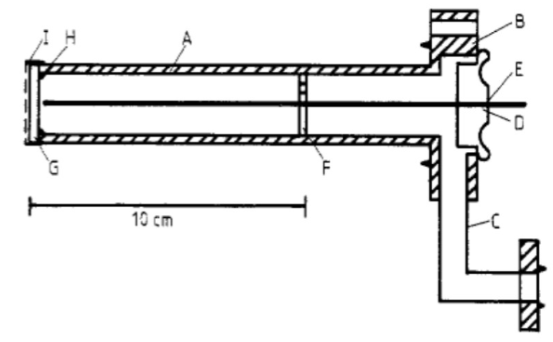
\includegraphics[scale=0.45]{Figs/tubedesign.png}
\end{frame}

\subsection{Research Goals}
\begin{frame}{Research Goals}
    \begin{itemize}
        \item Explore the count rates of the tubes as a function of different acetone pressures and anode voltages
        \item Find regions which give us the maximum count rates (catching the most photons)
        \item The region must be stable, meaning no tube breakdowns (self arcing) 
    \end{itemize}
\end{frame}

\section{Experimental Design}

\subsection{Experimental Setup}
\begin{frame}{Experimental Setup}
    \begin{itemize}
        \item Sample is mounted in front of an electron gun in an UHV chamber, it is important to ground the sample to prevent charge buildup 
        \item The GM tubes are on either side of the electron gun, focusing on the sample
        \item The tubes are mutually connected to a gas manifold for filling and evacuating, and separately connected to a preamplifier and high voltage power supply
        \item The output of the preamplifier is connected to a shaping amplifier to convert the signal to a gaussian pulse, and finally the shaping amplifier is connected to a MCA 
        which is interfaced with a pc
    \end{itemize}
\end{frame}

\begin{frame}{Types of Signals}
    \centering
    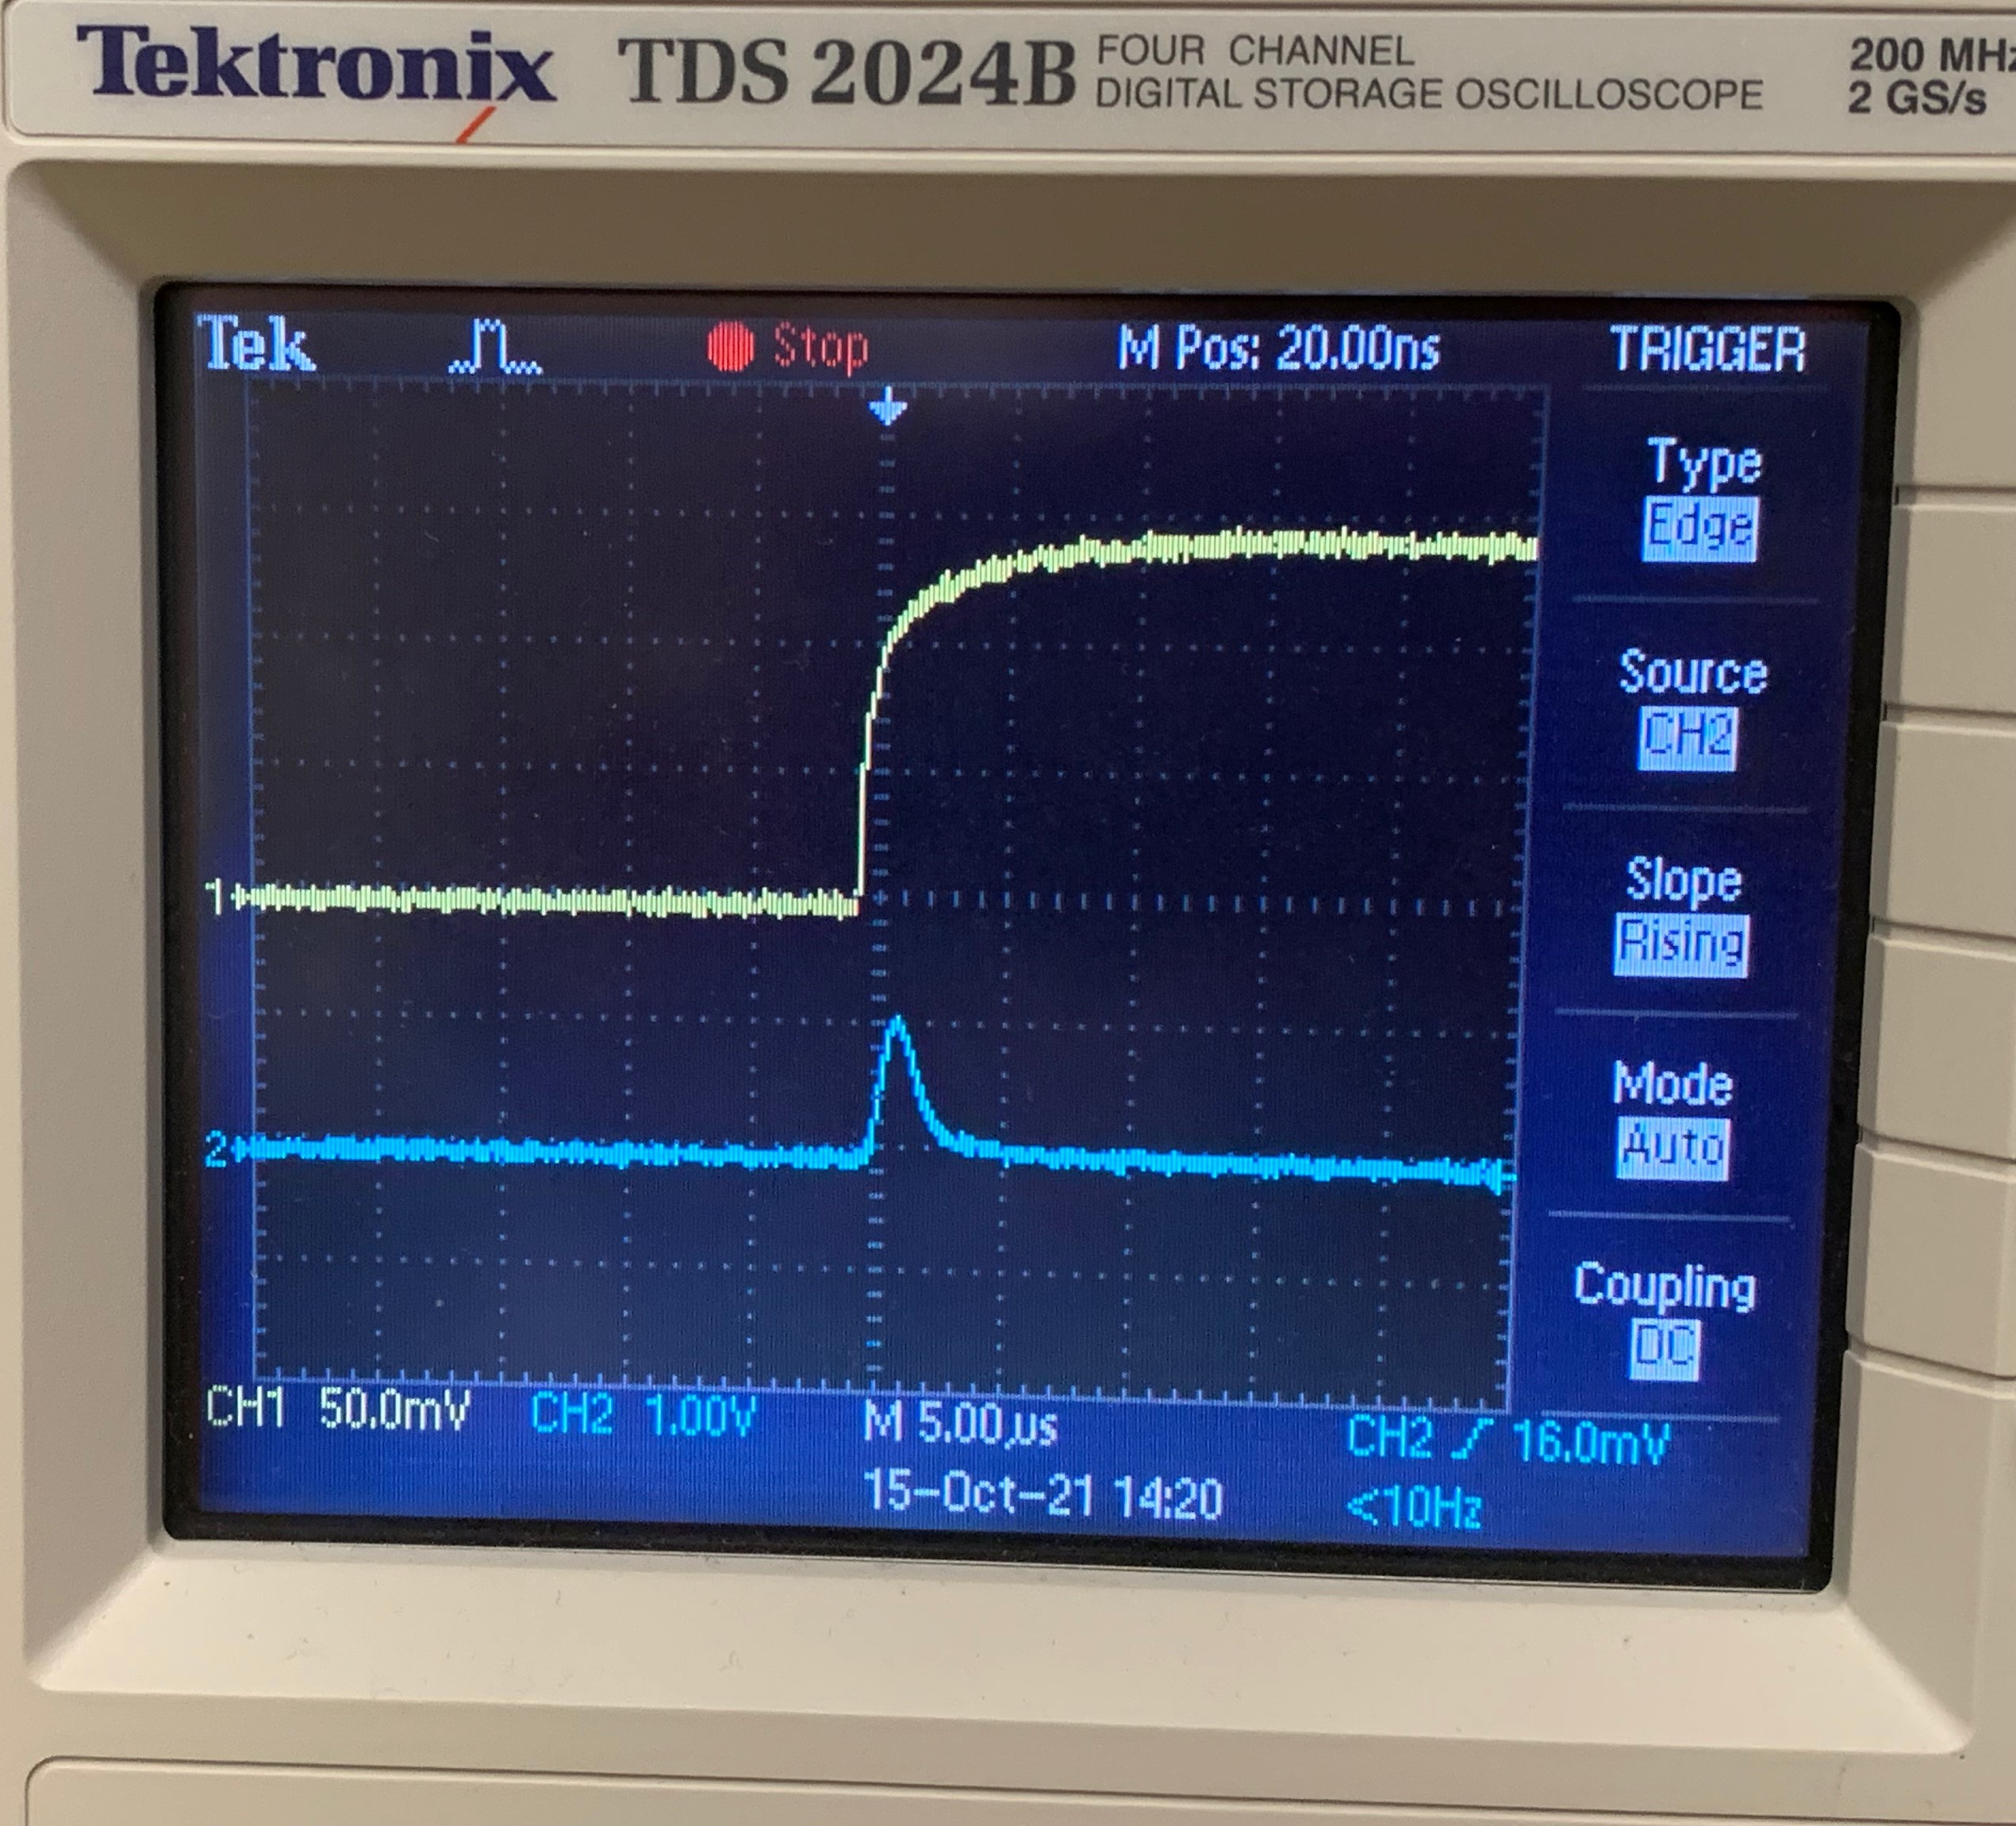
\includegraphics[scale=0.14]{Figs/pulses.png}
\end{frame}

\subsection{Procedure}
\begin{frame}{Procedure}
    \begin{itemize}
        \item Start by evacuating the tubes, do this because tube breakdown cracks acetone gas making it useless for photon detection 
        \item Fill the tubes to desired pressure using a needle valve attached to a cylinder of acetone
        \item Run scanning program which sets anode voltage, measures the count rate with the electron gun off, then turns gun on and measures count rate again. Iterates the process 
        over a set range of anode voltages 
        \item Use gun off data to identify the voltage at which breakdown starts to occur (label this the breakdown voltage)
        \item Examine the count rates only below the breakdown voltage 
    \end{itemize}
\end{frame}

\section{Results}

\begin{frame}{Left Tube}
    \begin{figure}[h!]
        \centering
        \subcaptionbox*{}[0.49\linewidth]{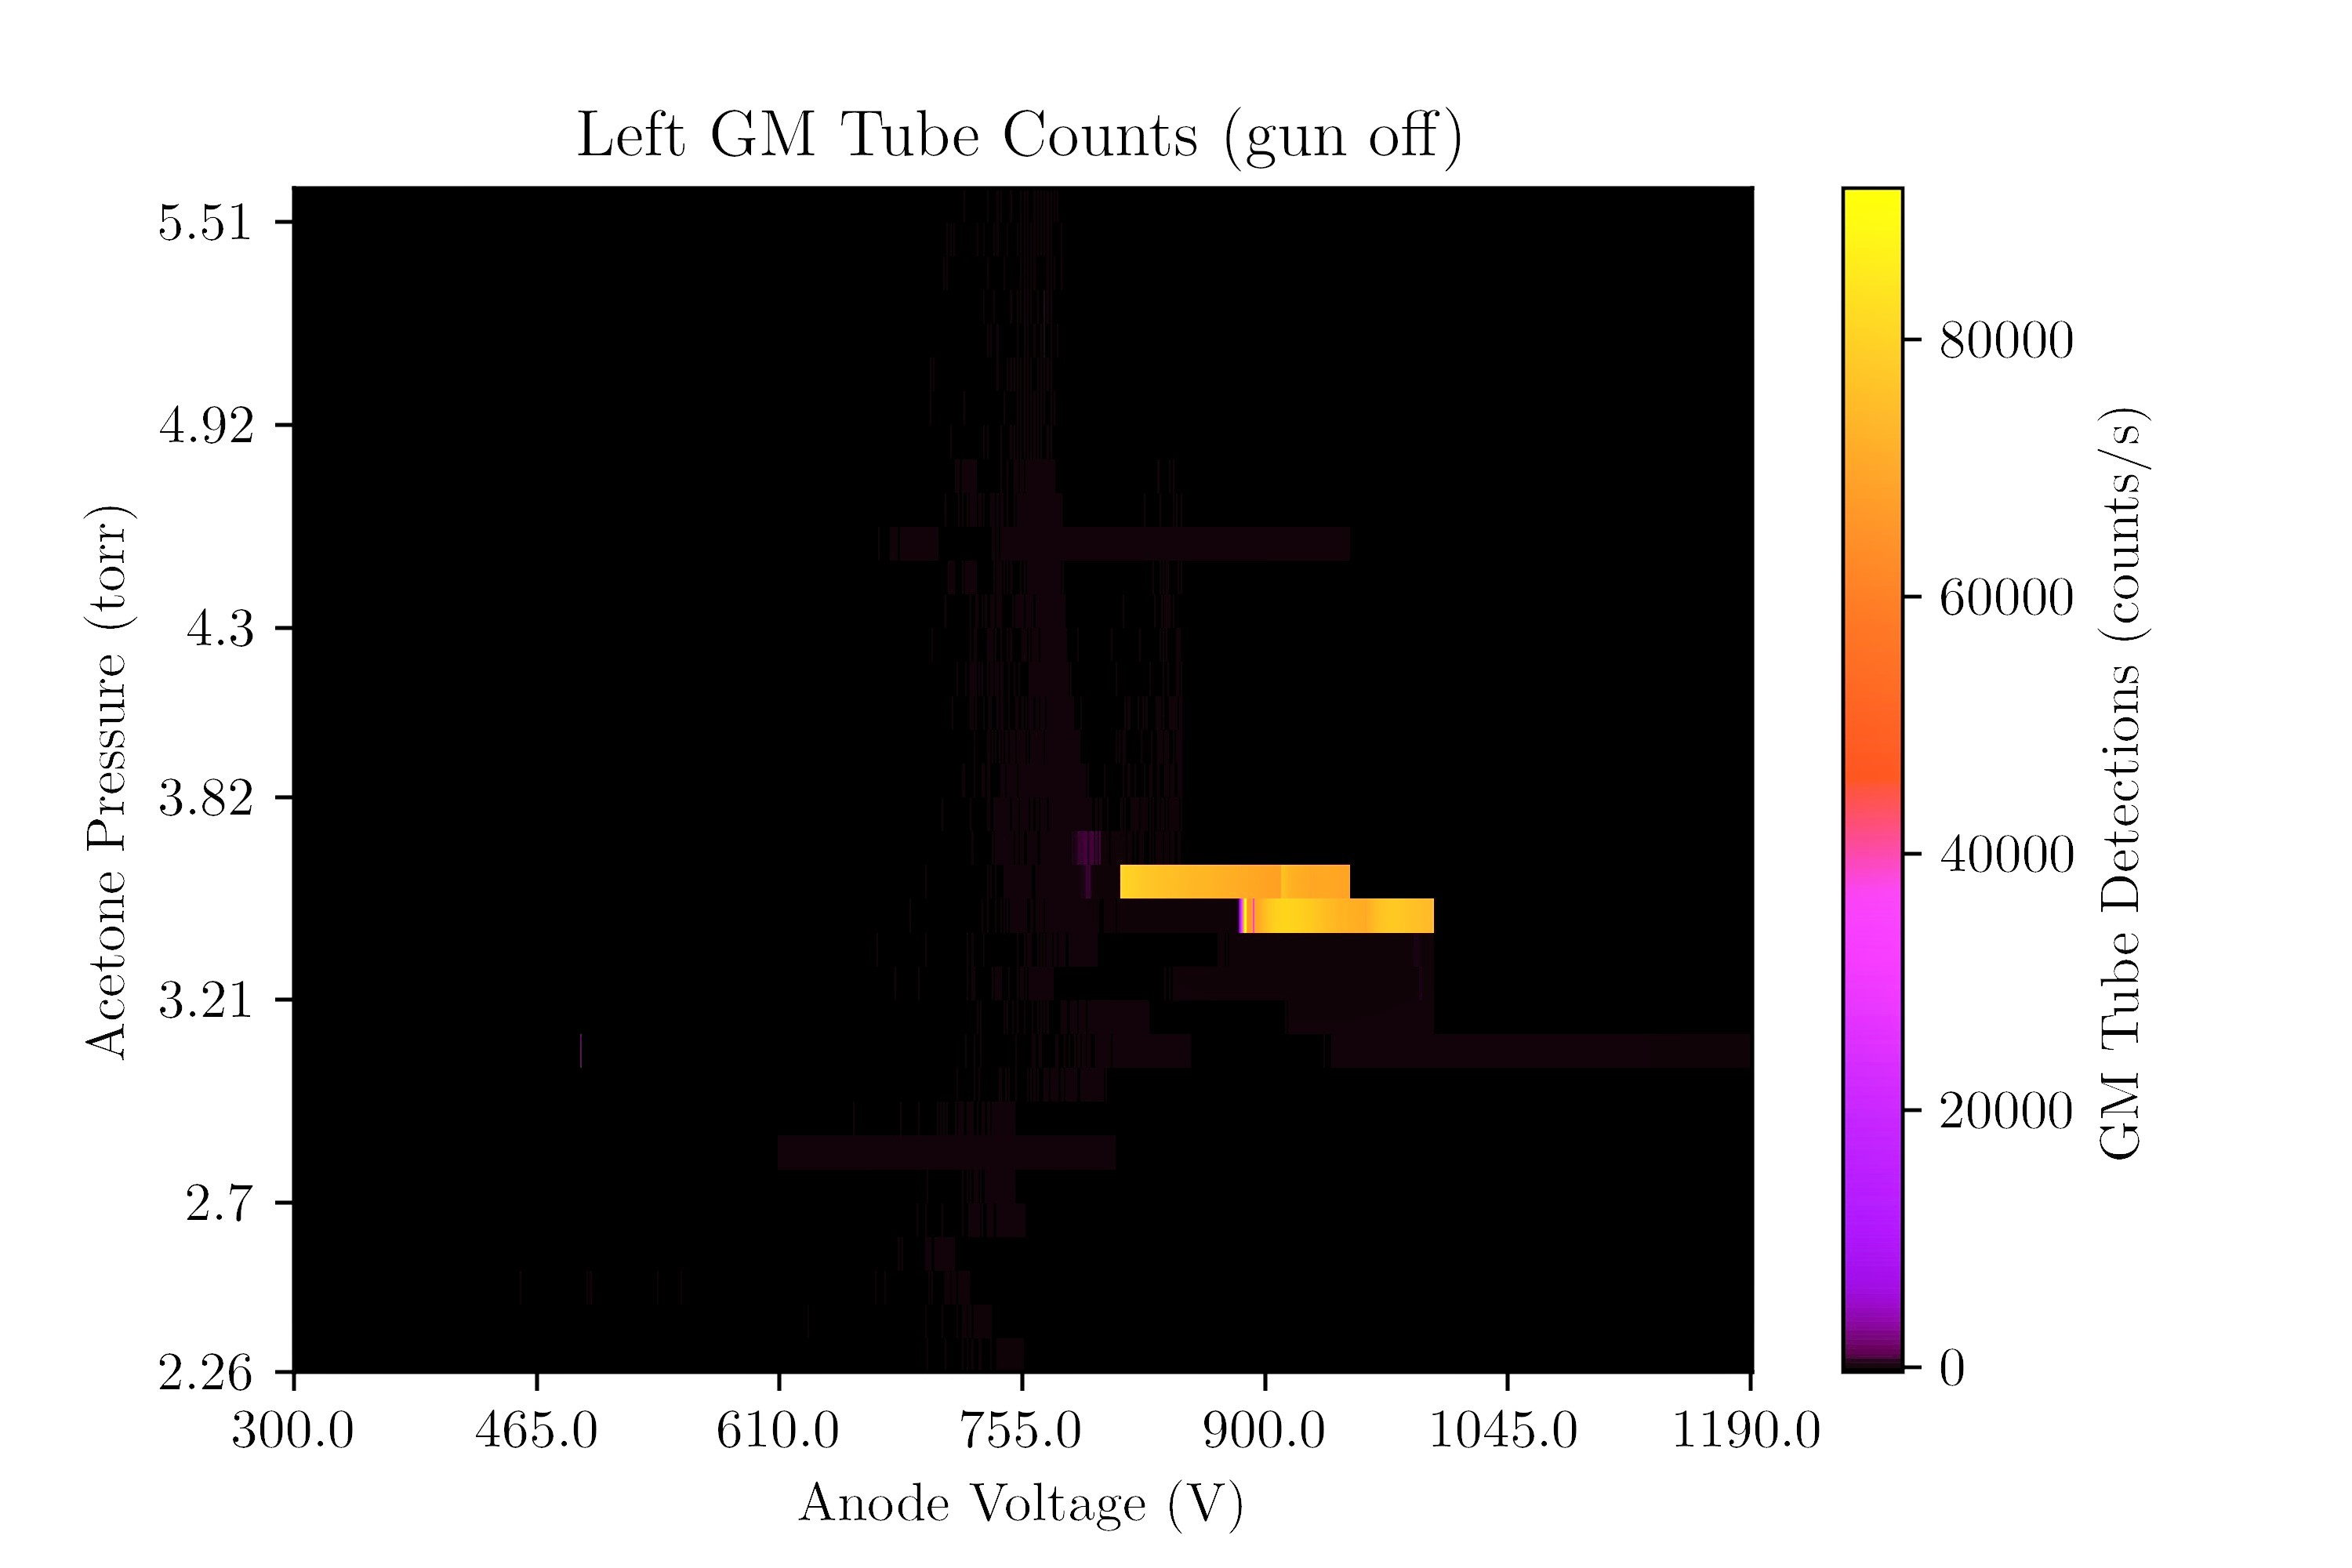
\includegraphics[scale=0.45]{Figs/LGMGunOff.jpg}}
        \subcaptionbox*{}[0.49\linewidth]{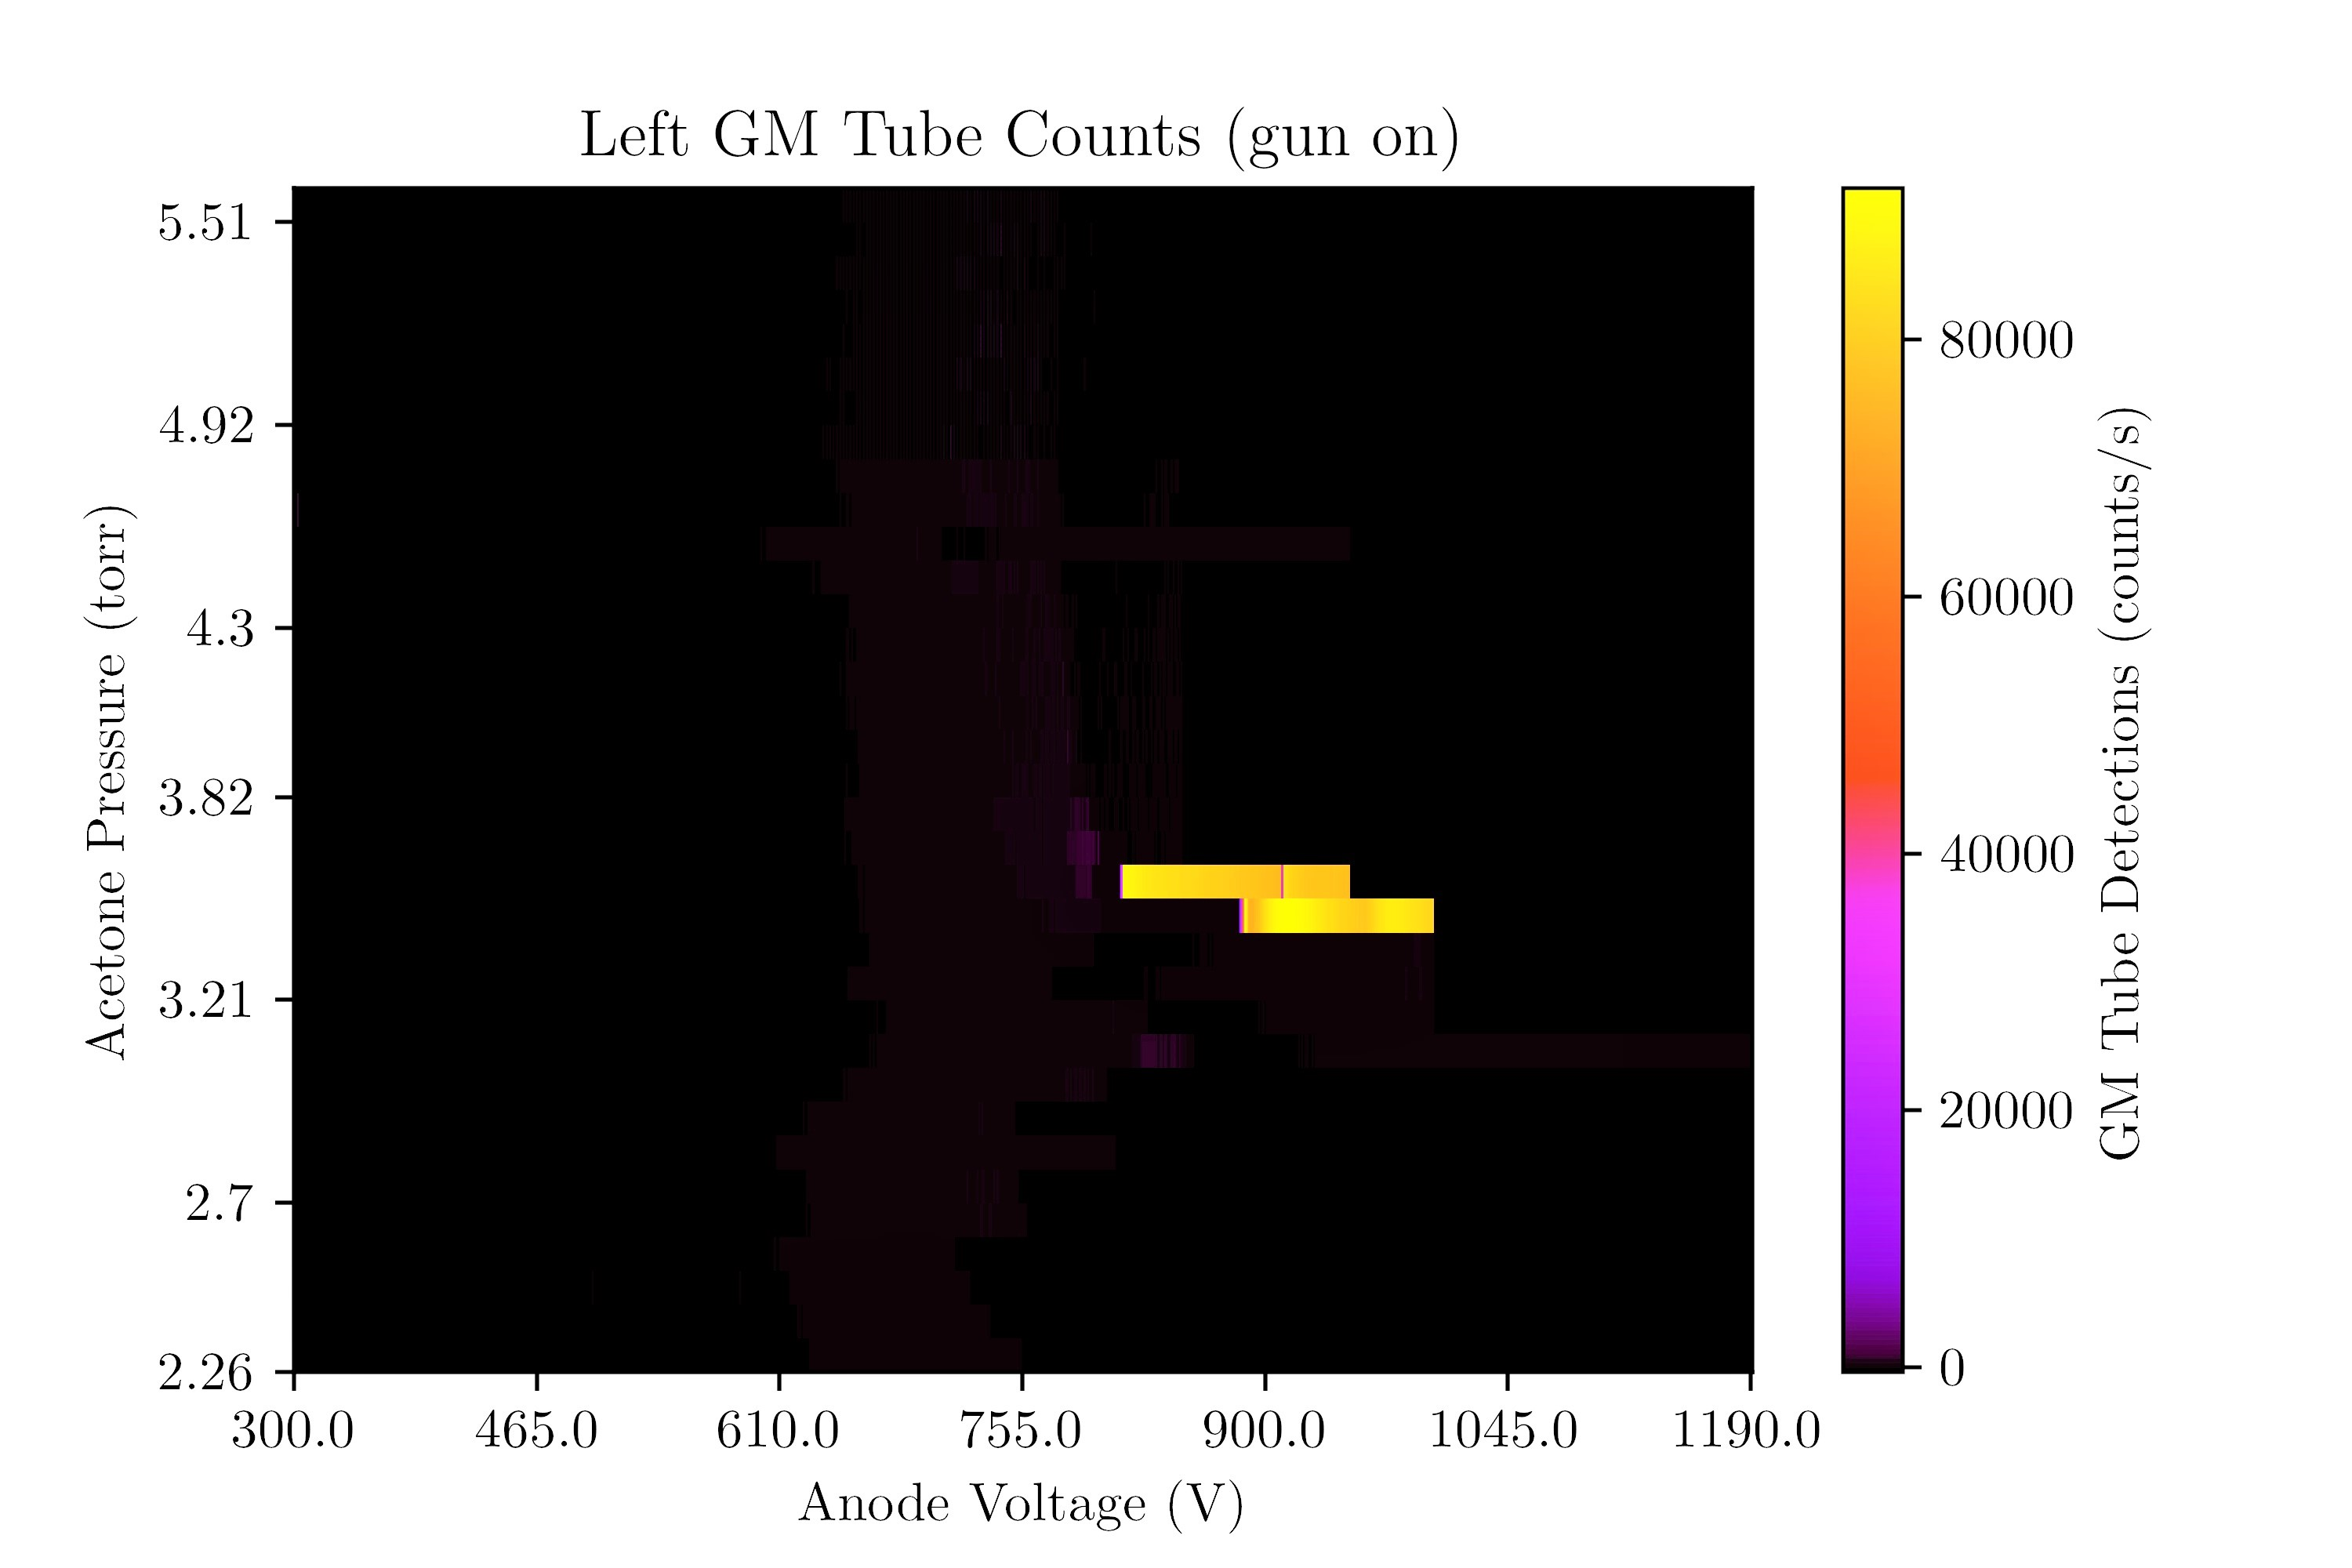
\includegraphics[scale=0.45]{Figs/LGMGunOn.jpg}}
    \end{figure}
\end{frame}

\begin{frame}{Right Tube}
    \begin{figure}[h!]
        \centering
        \subcaptionbox*{}[0.49\linewidth]{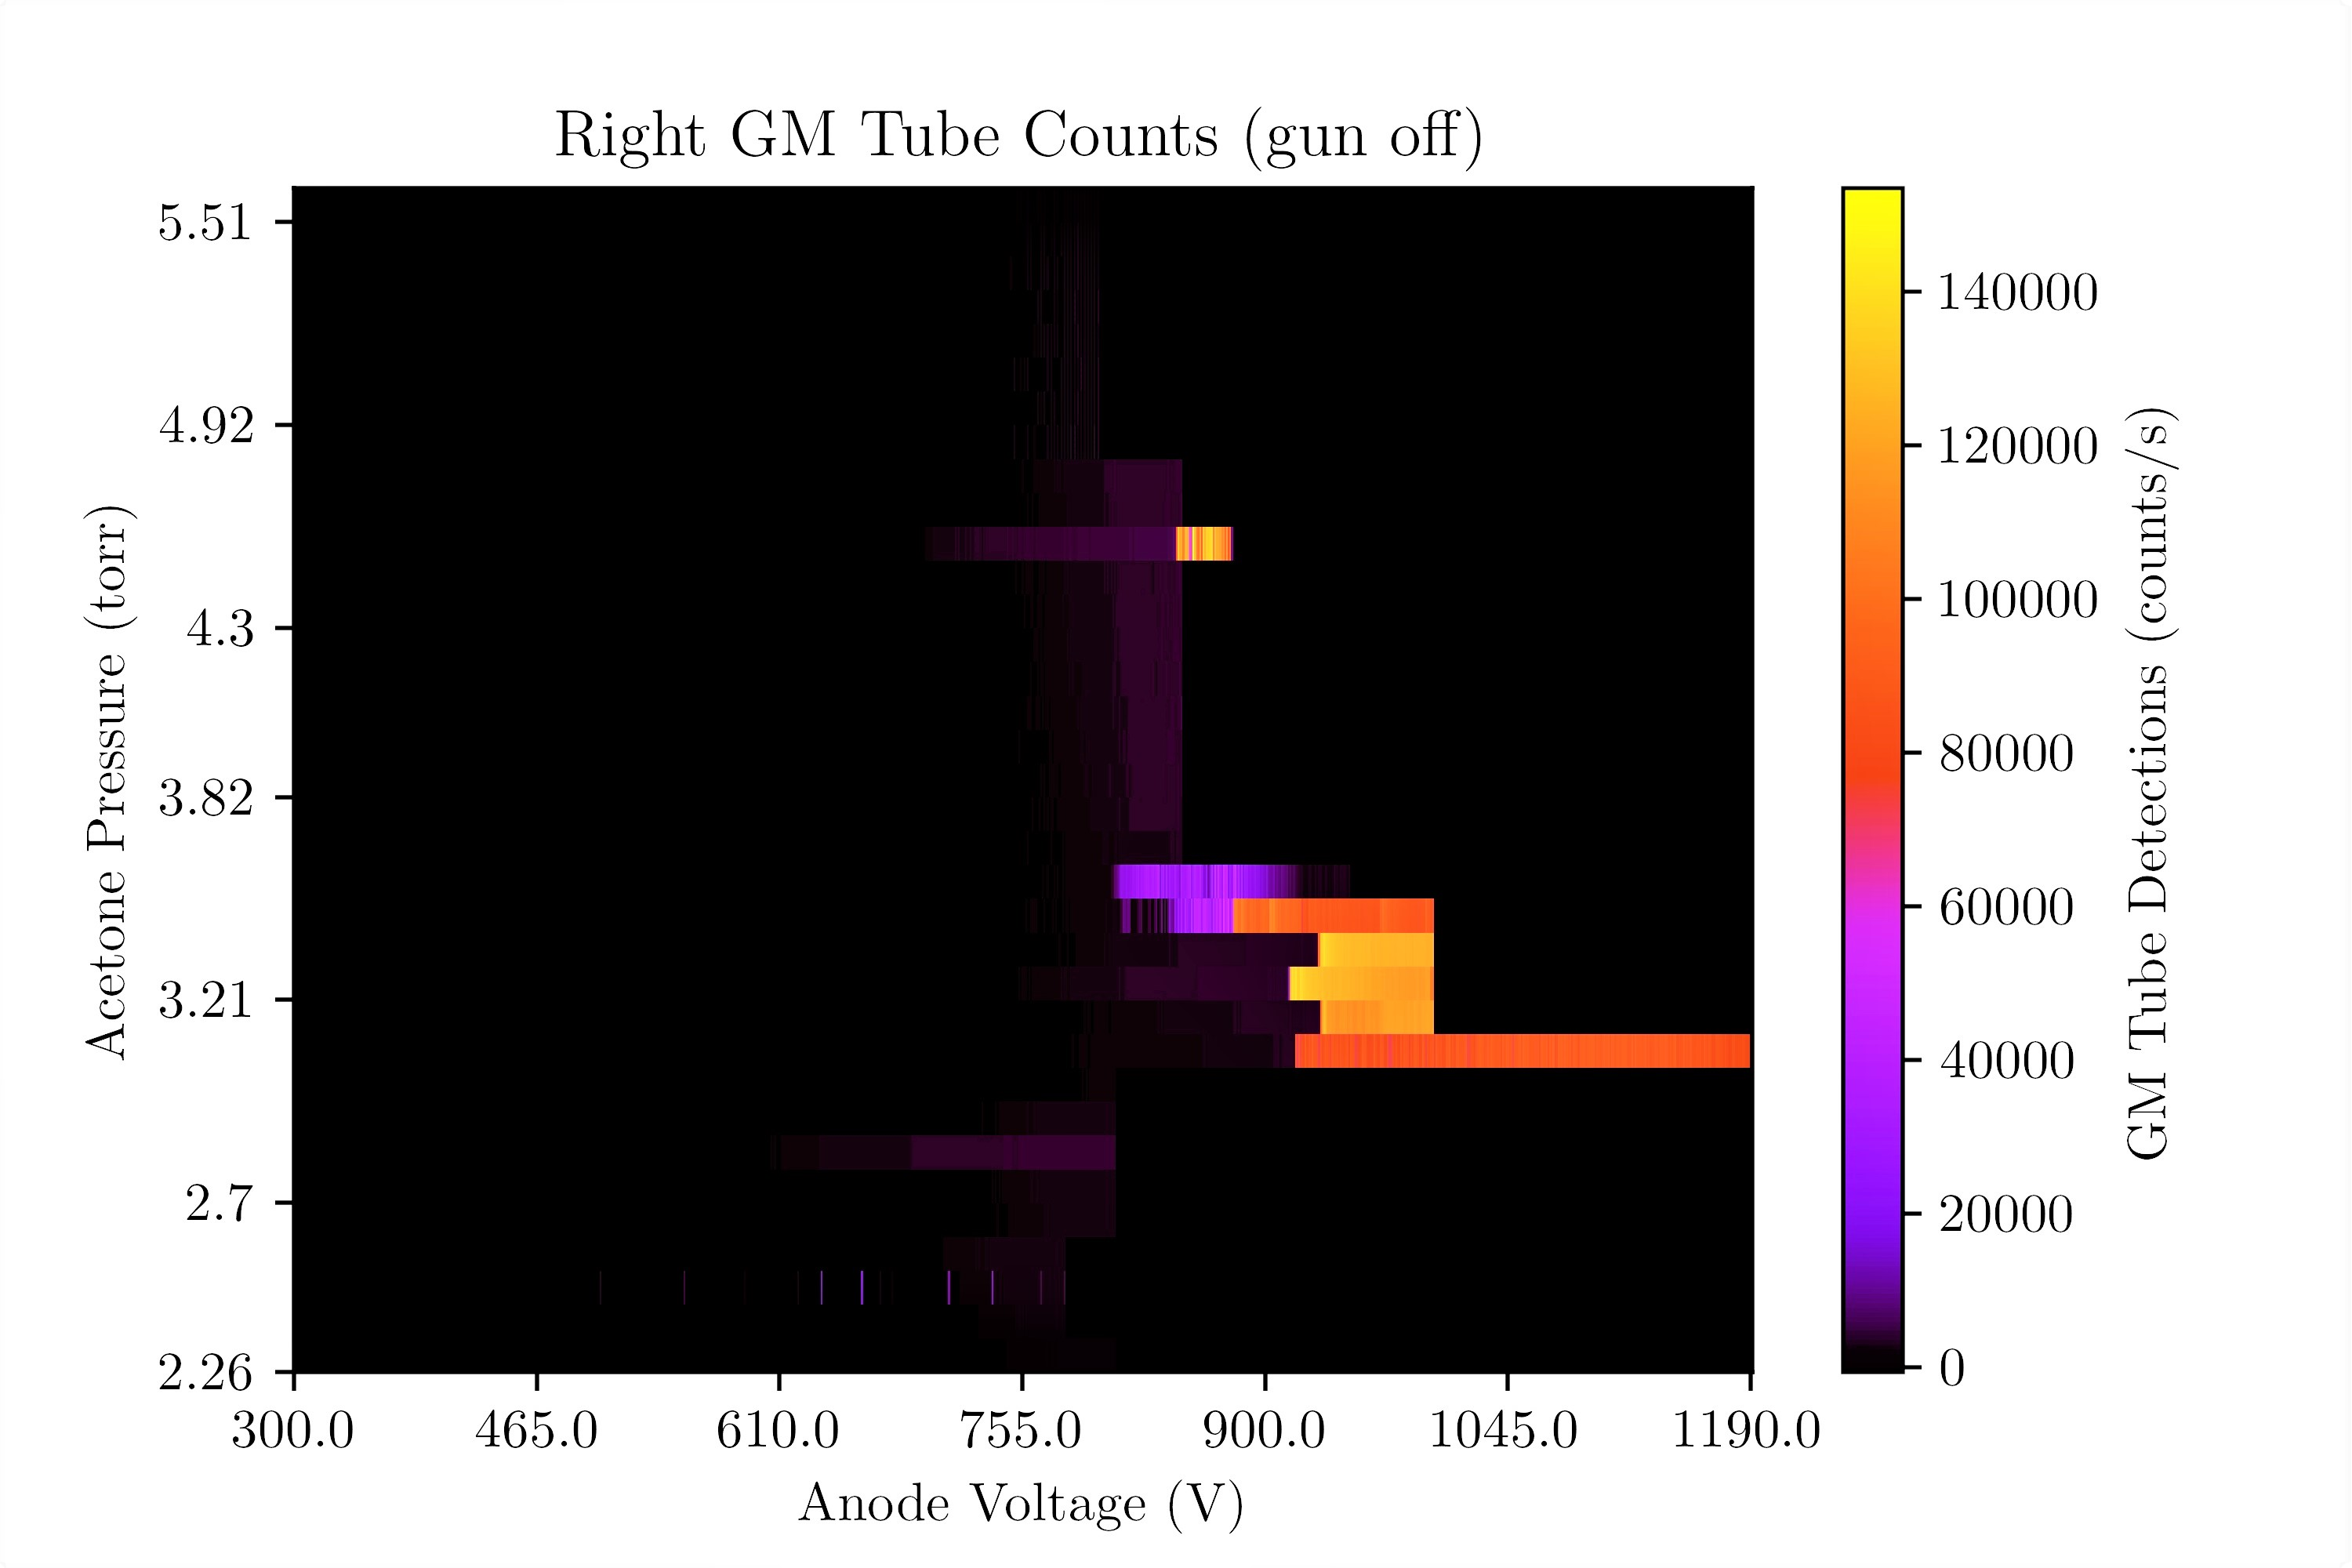
\includegraphics[scale=0.45]{Figs/RGMGunOff.jpg}}
        \subcaptionbox*{}[0.49\linewidth]{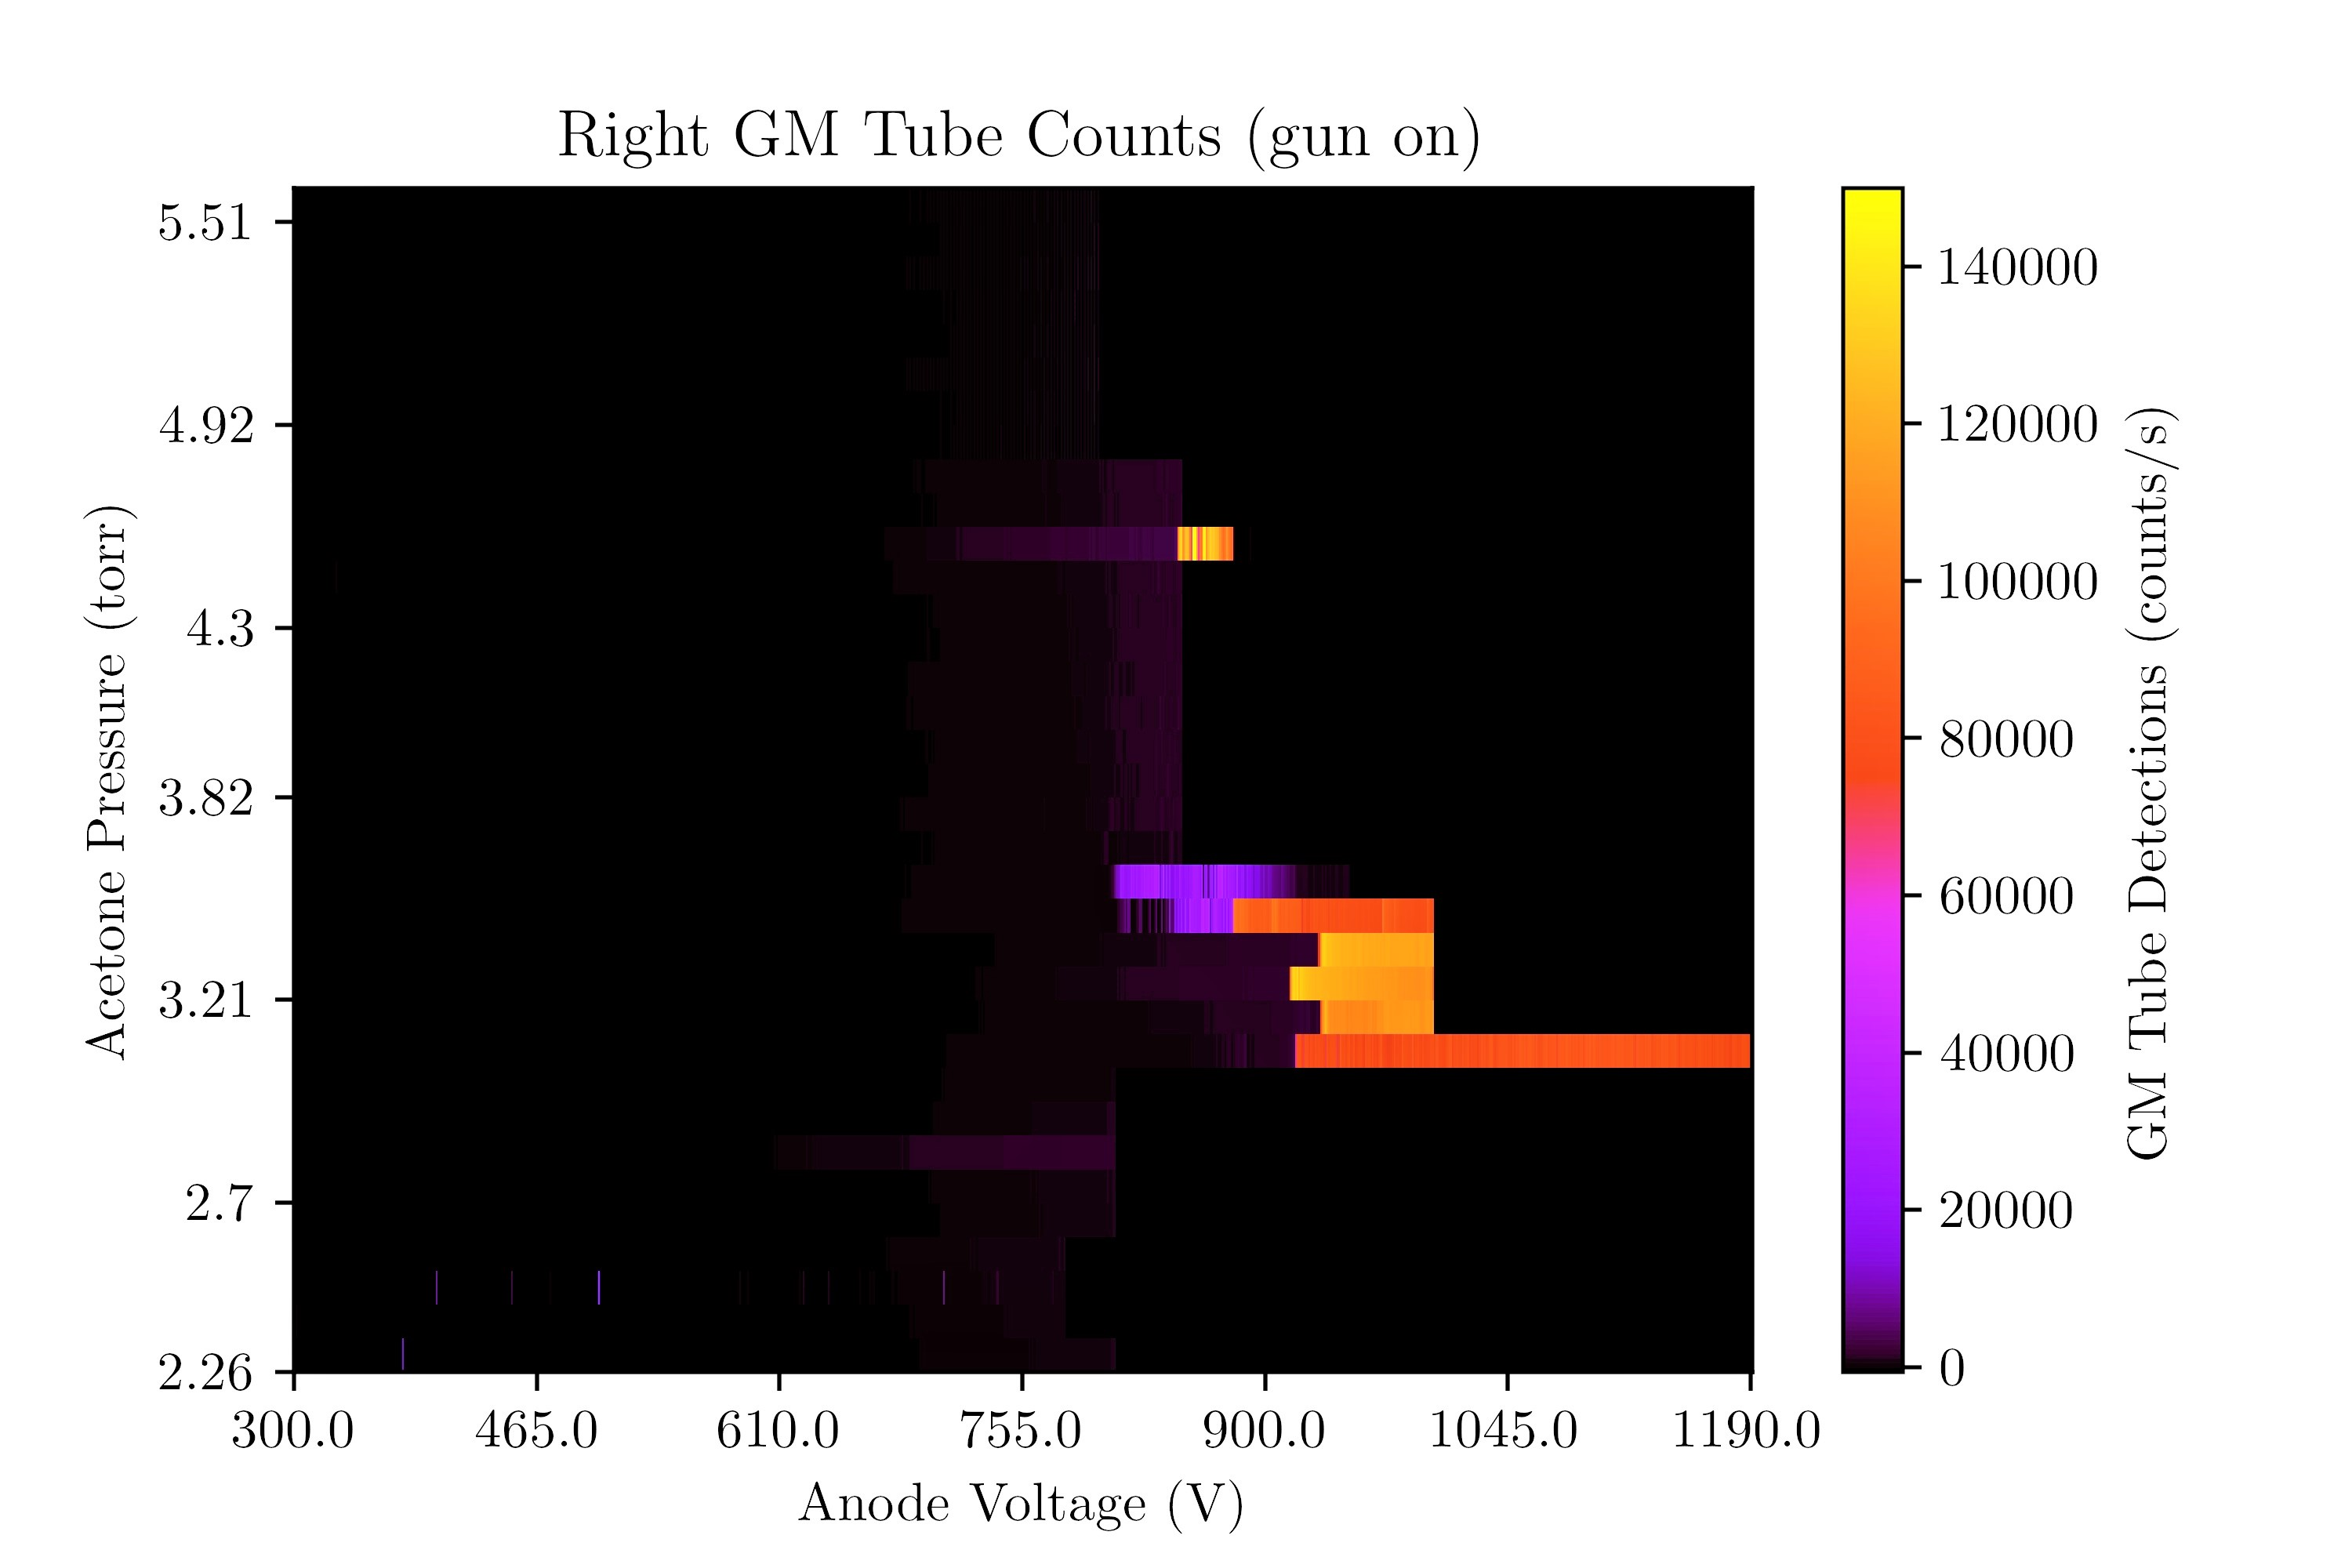
\includegraphics[scale=0.45]{Figs/RGMGunOn.jpg}}
    \end{figure}
\end{frame}

\begin{frame}{Breakdown Voltage}
    \centering
    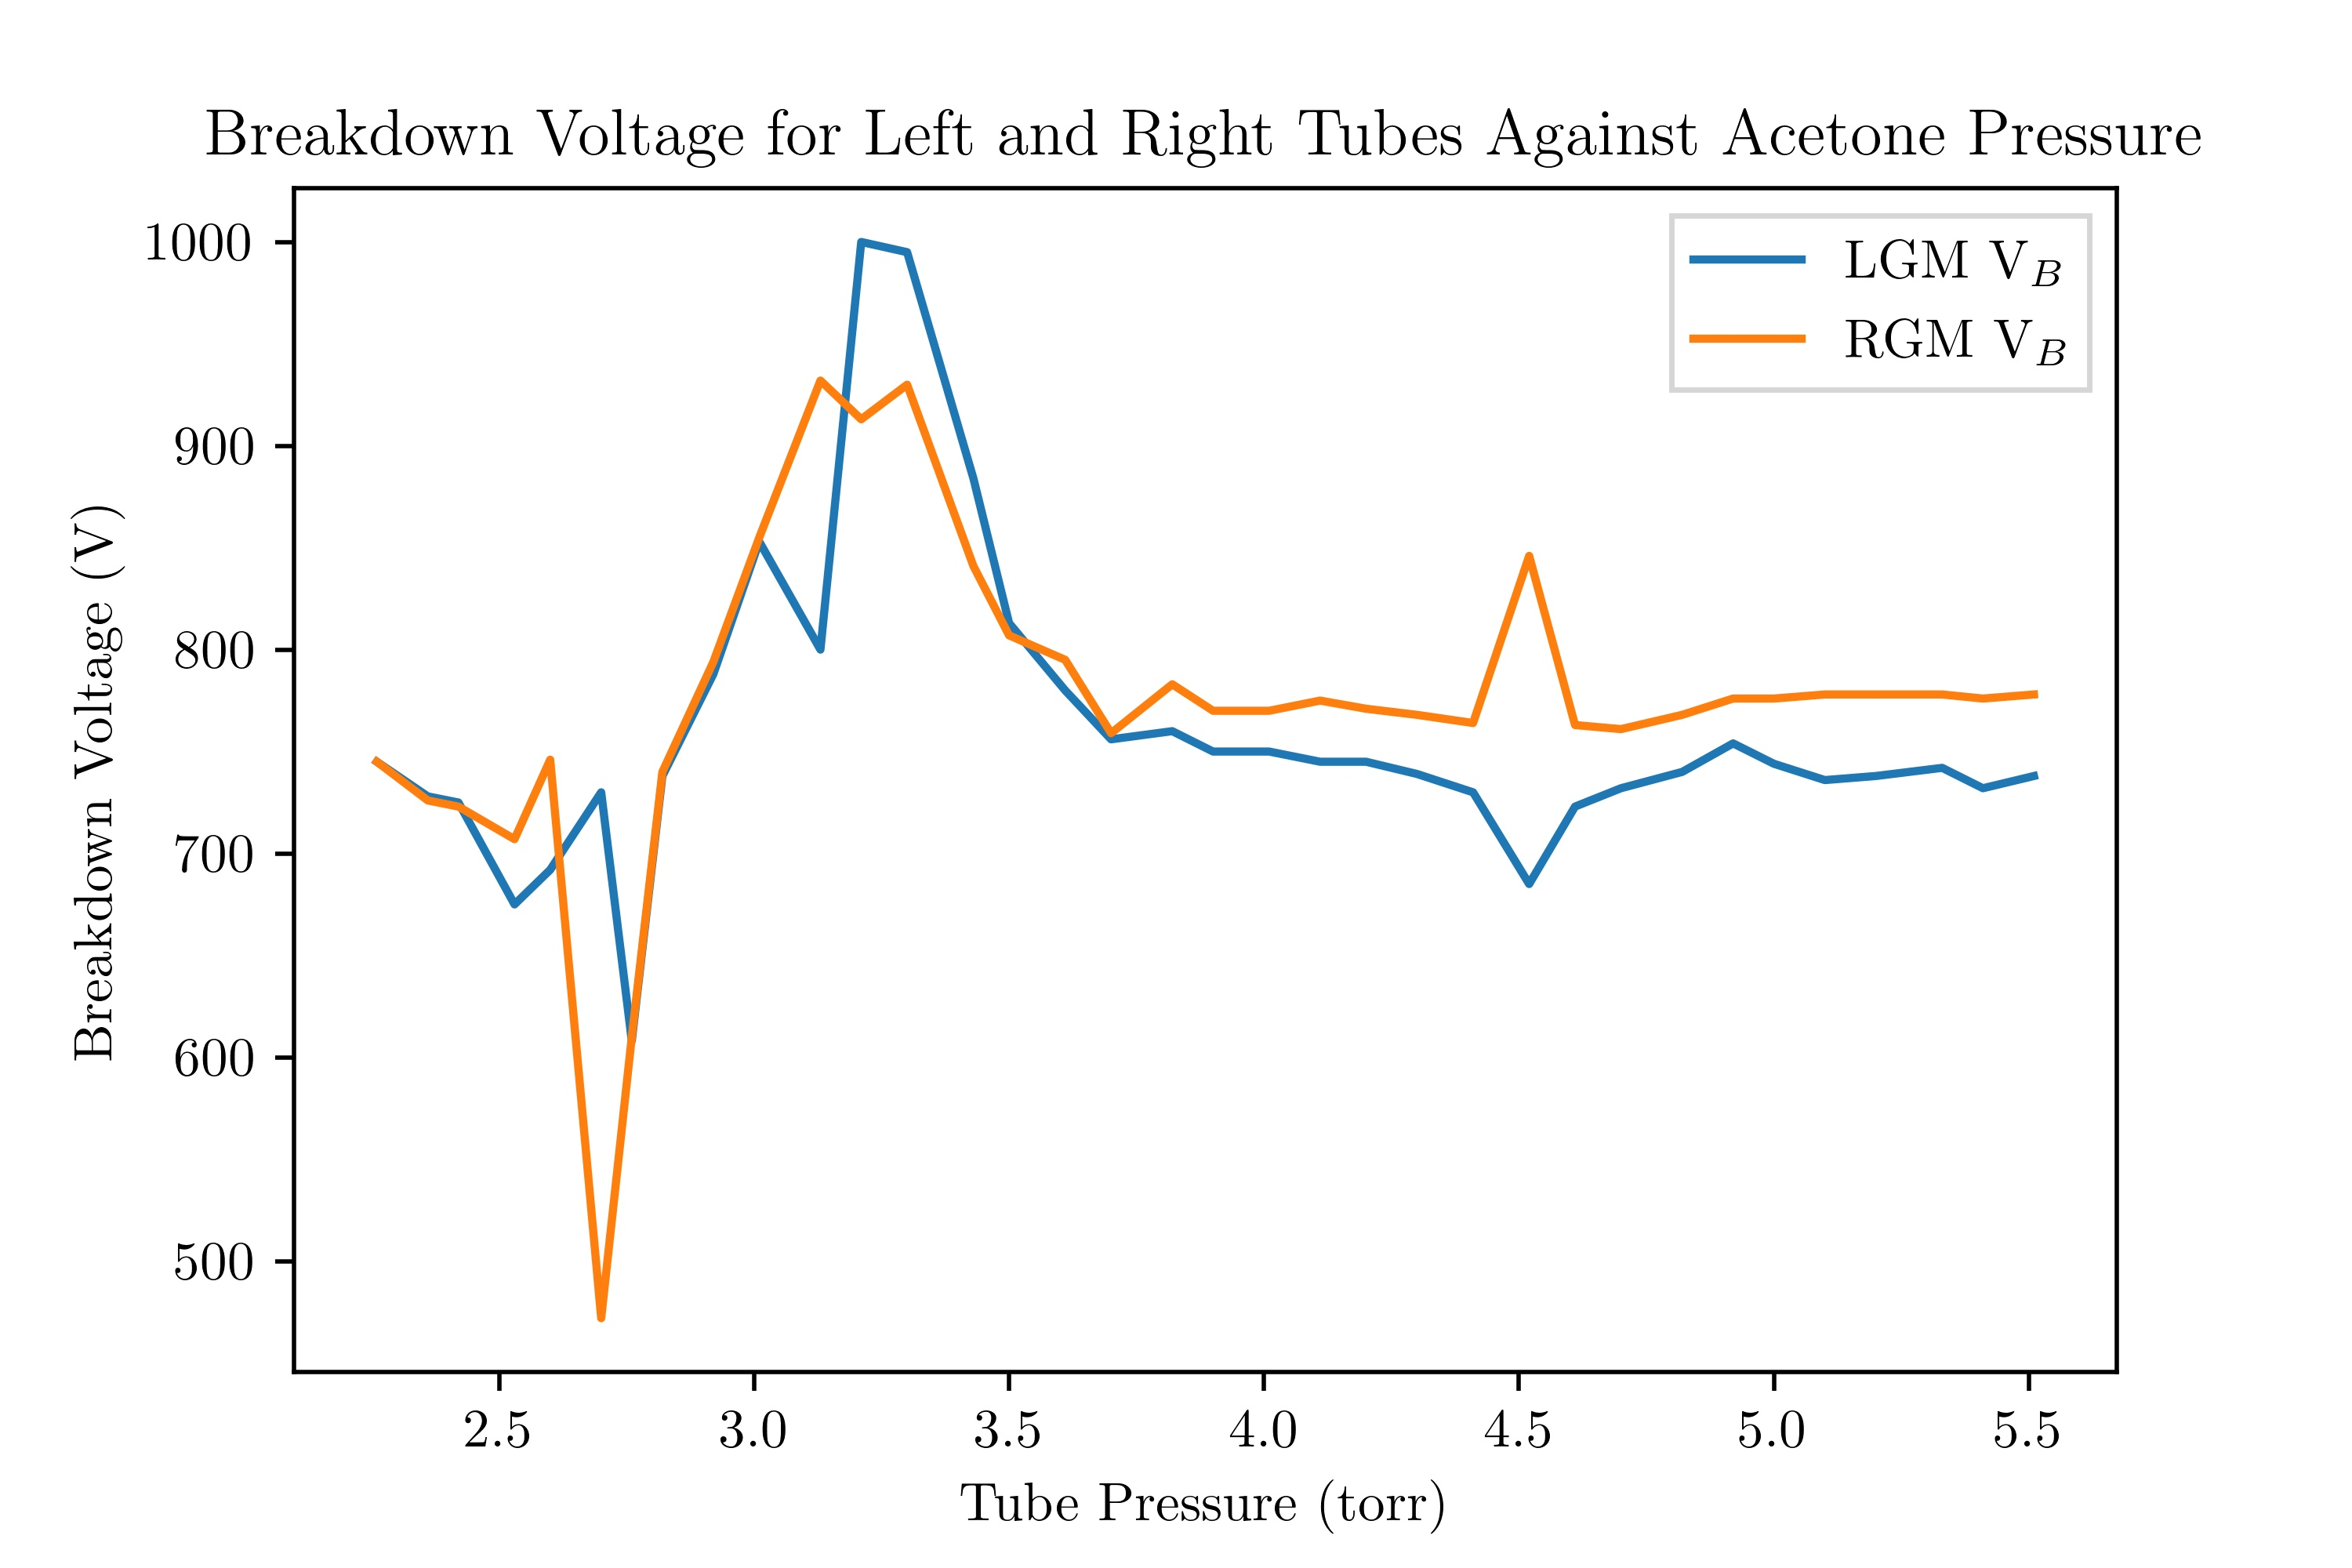
\includegraphics[scale=0.75]{Figs/VB.jpg}
\end{frame}

\begin{frame}{LGM Below $V_B$}
    \centering
    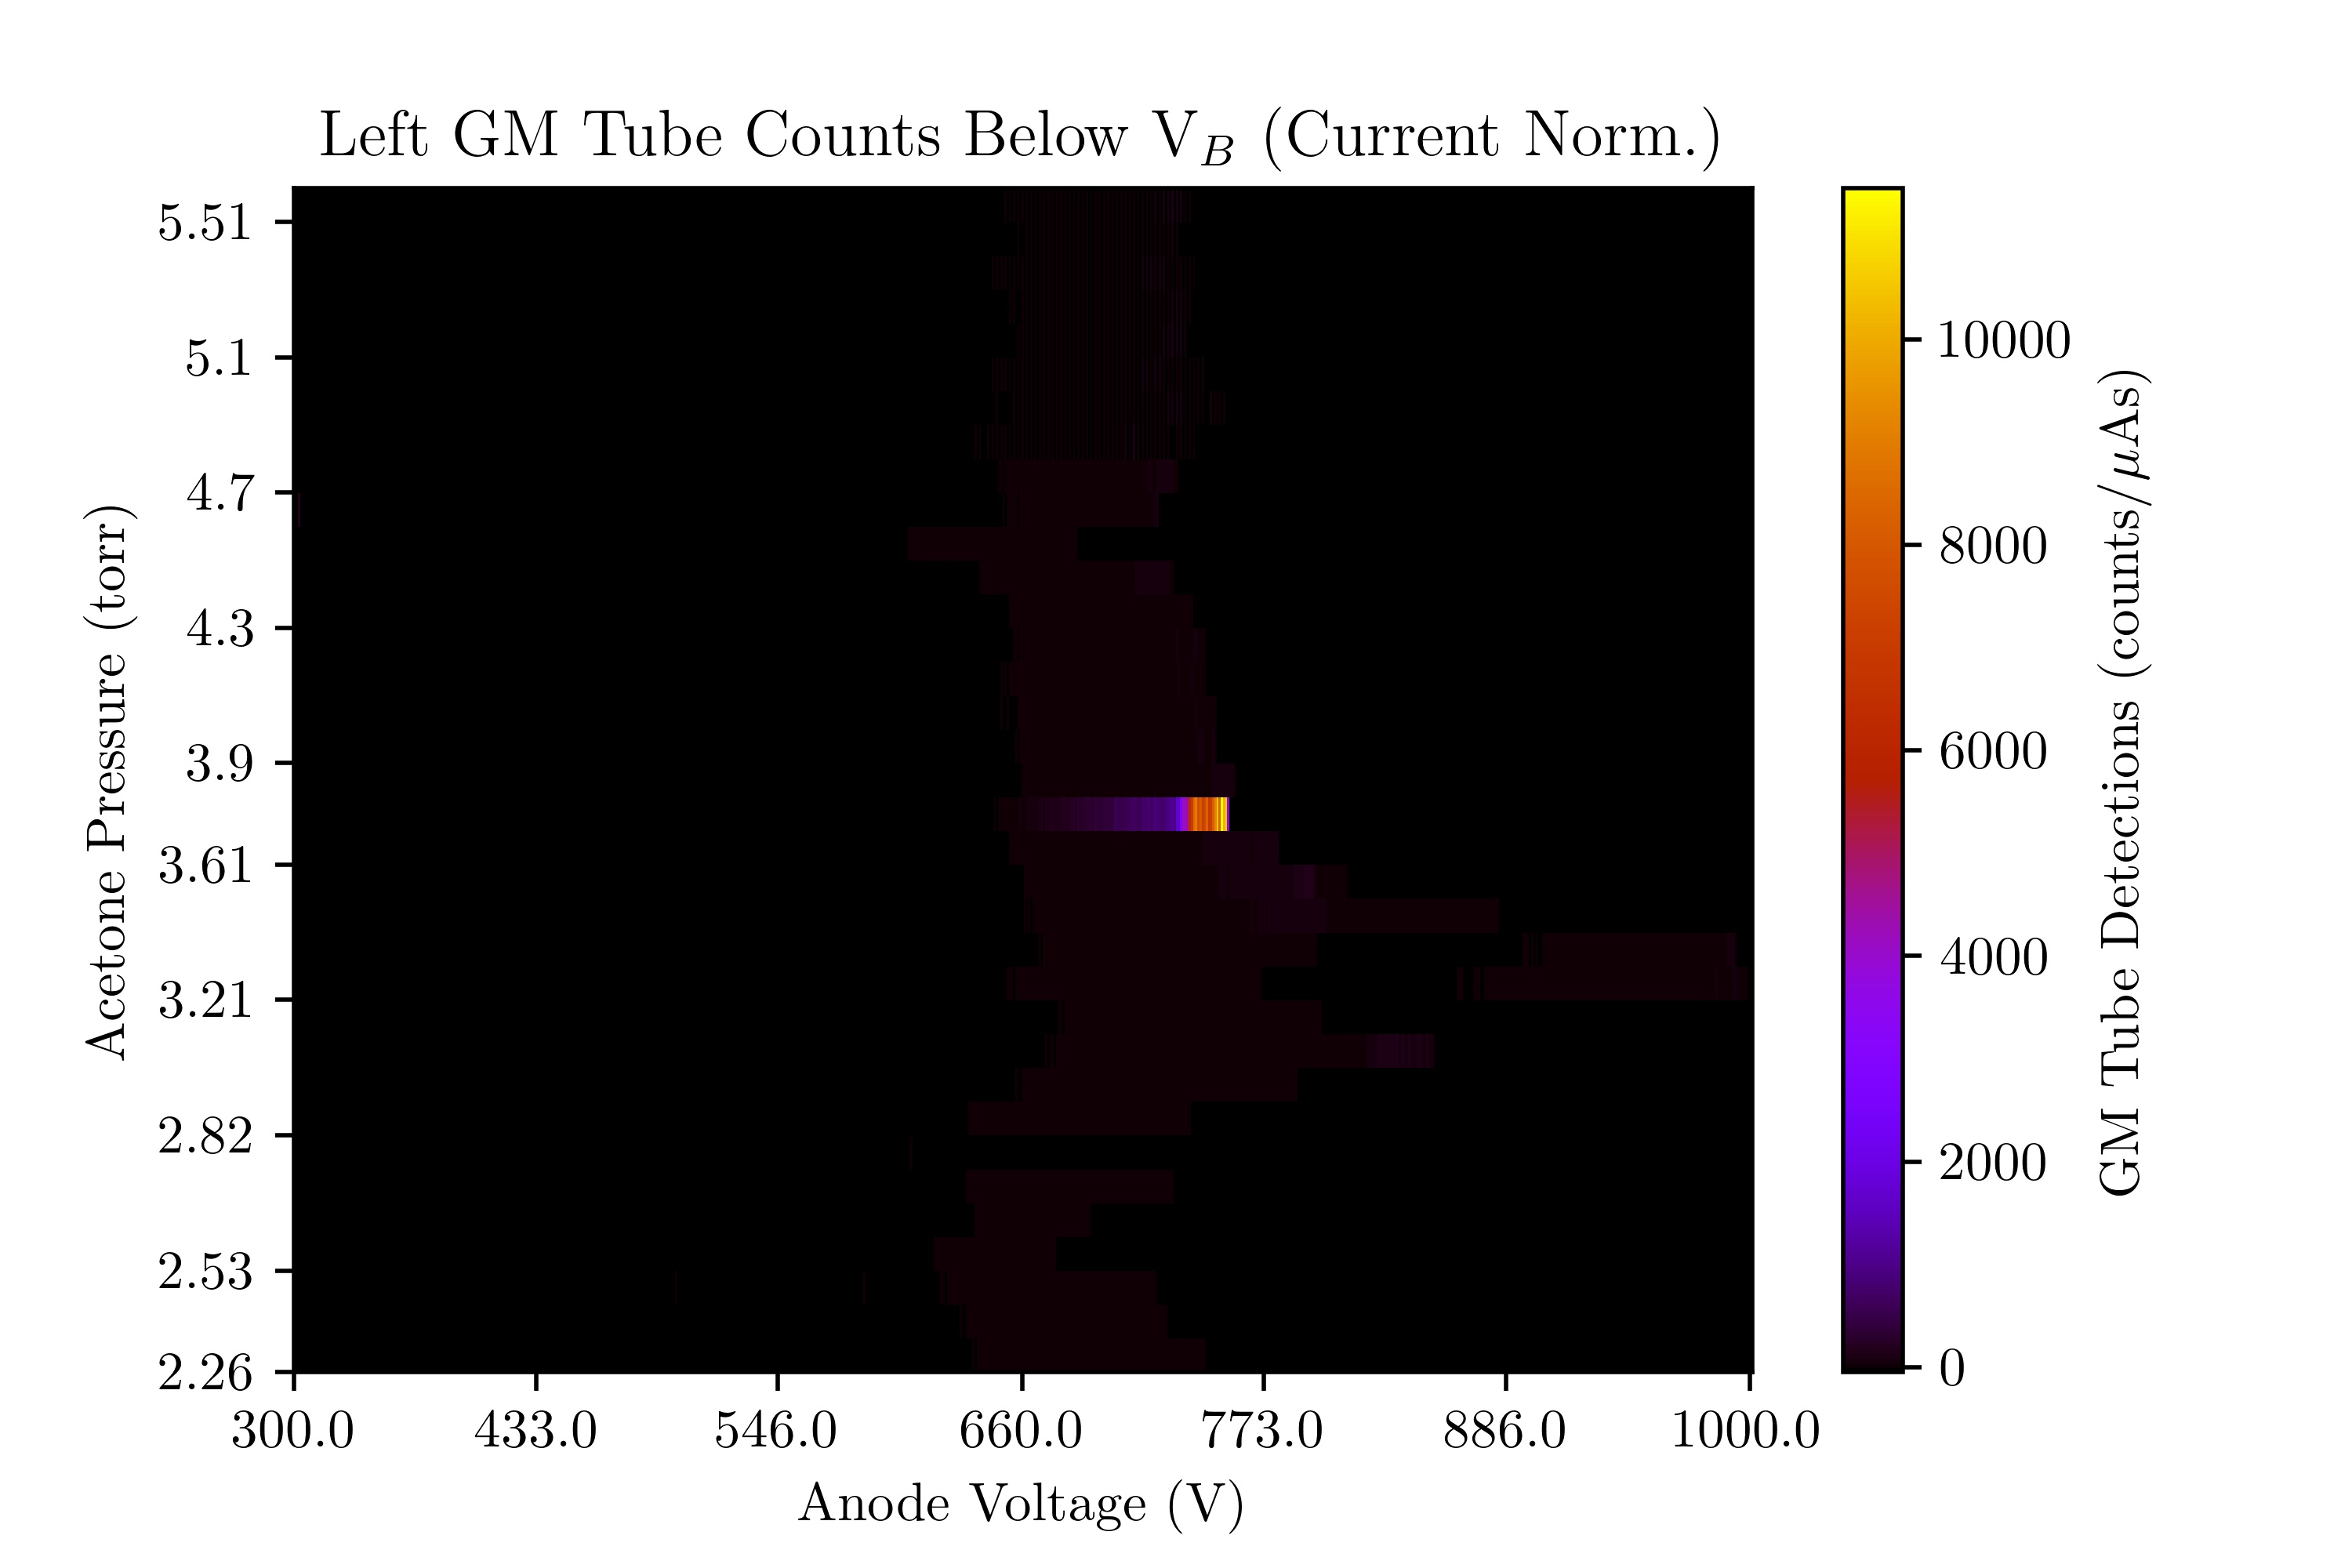
\includegraphics[scale=0.65]{Figs/LGMFinalNorm.jpg}\\
    Optimal pressure is 3.7 torr, optimal anode voltage is 740V
\end{frame}

\begin{frame}{LGM Cont.}
    \centering
    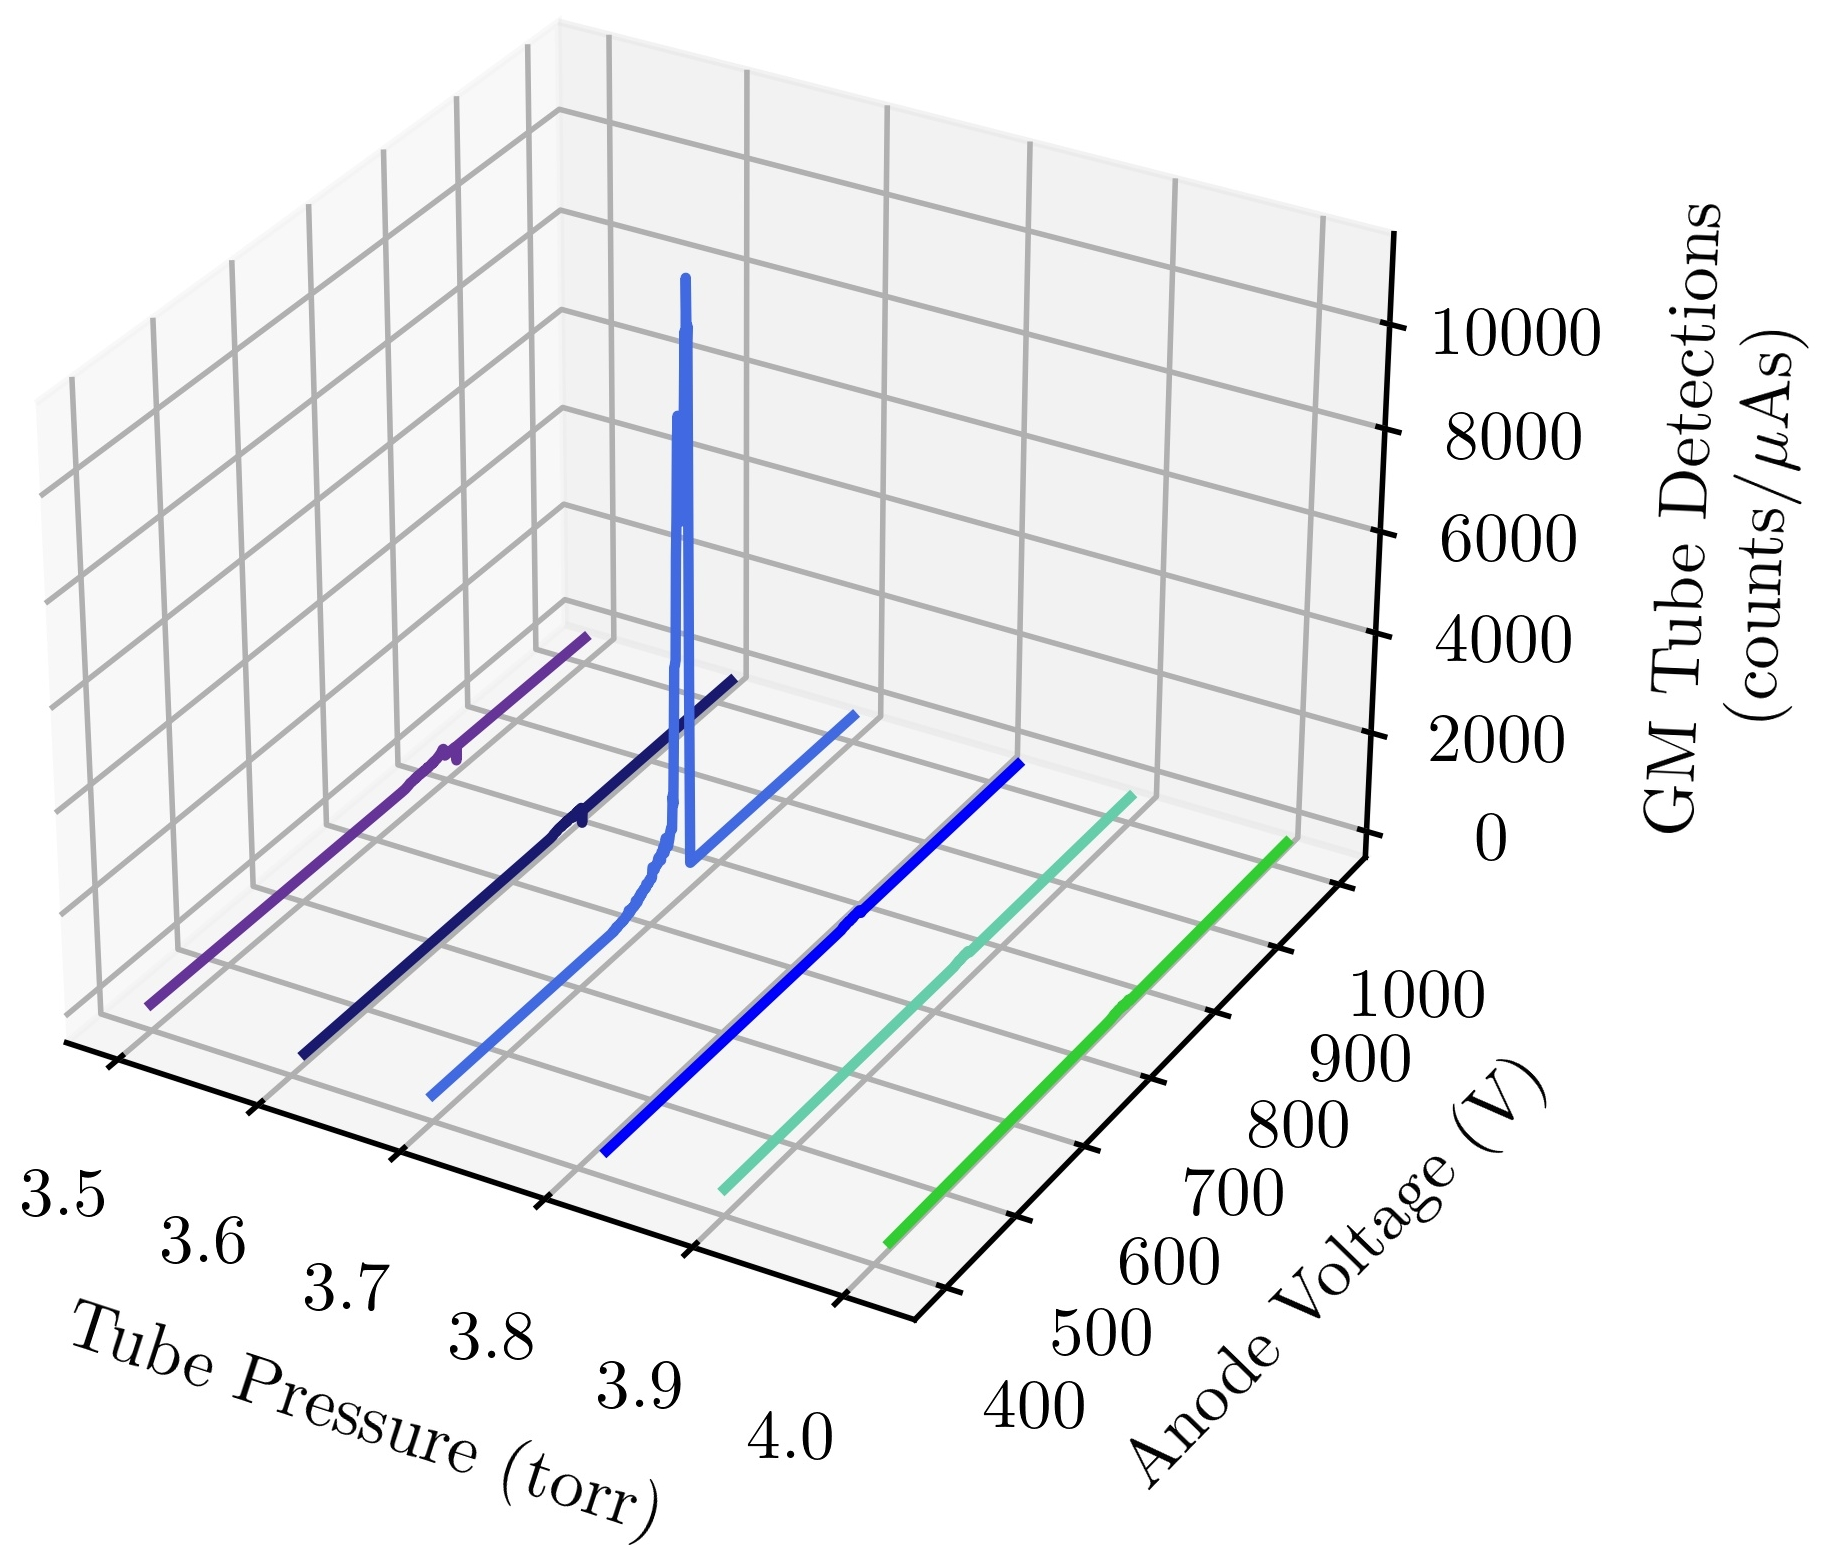
\includegraphics[scale=0.9]{Figs/Plots/LGM Waterfall.jpg}
\end{frame}

\begin{frame}{RGM Below $V_B$}
    \centering
    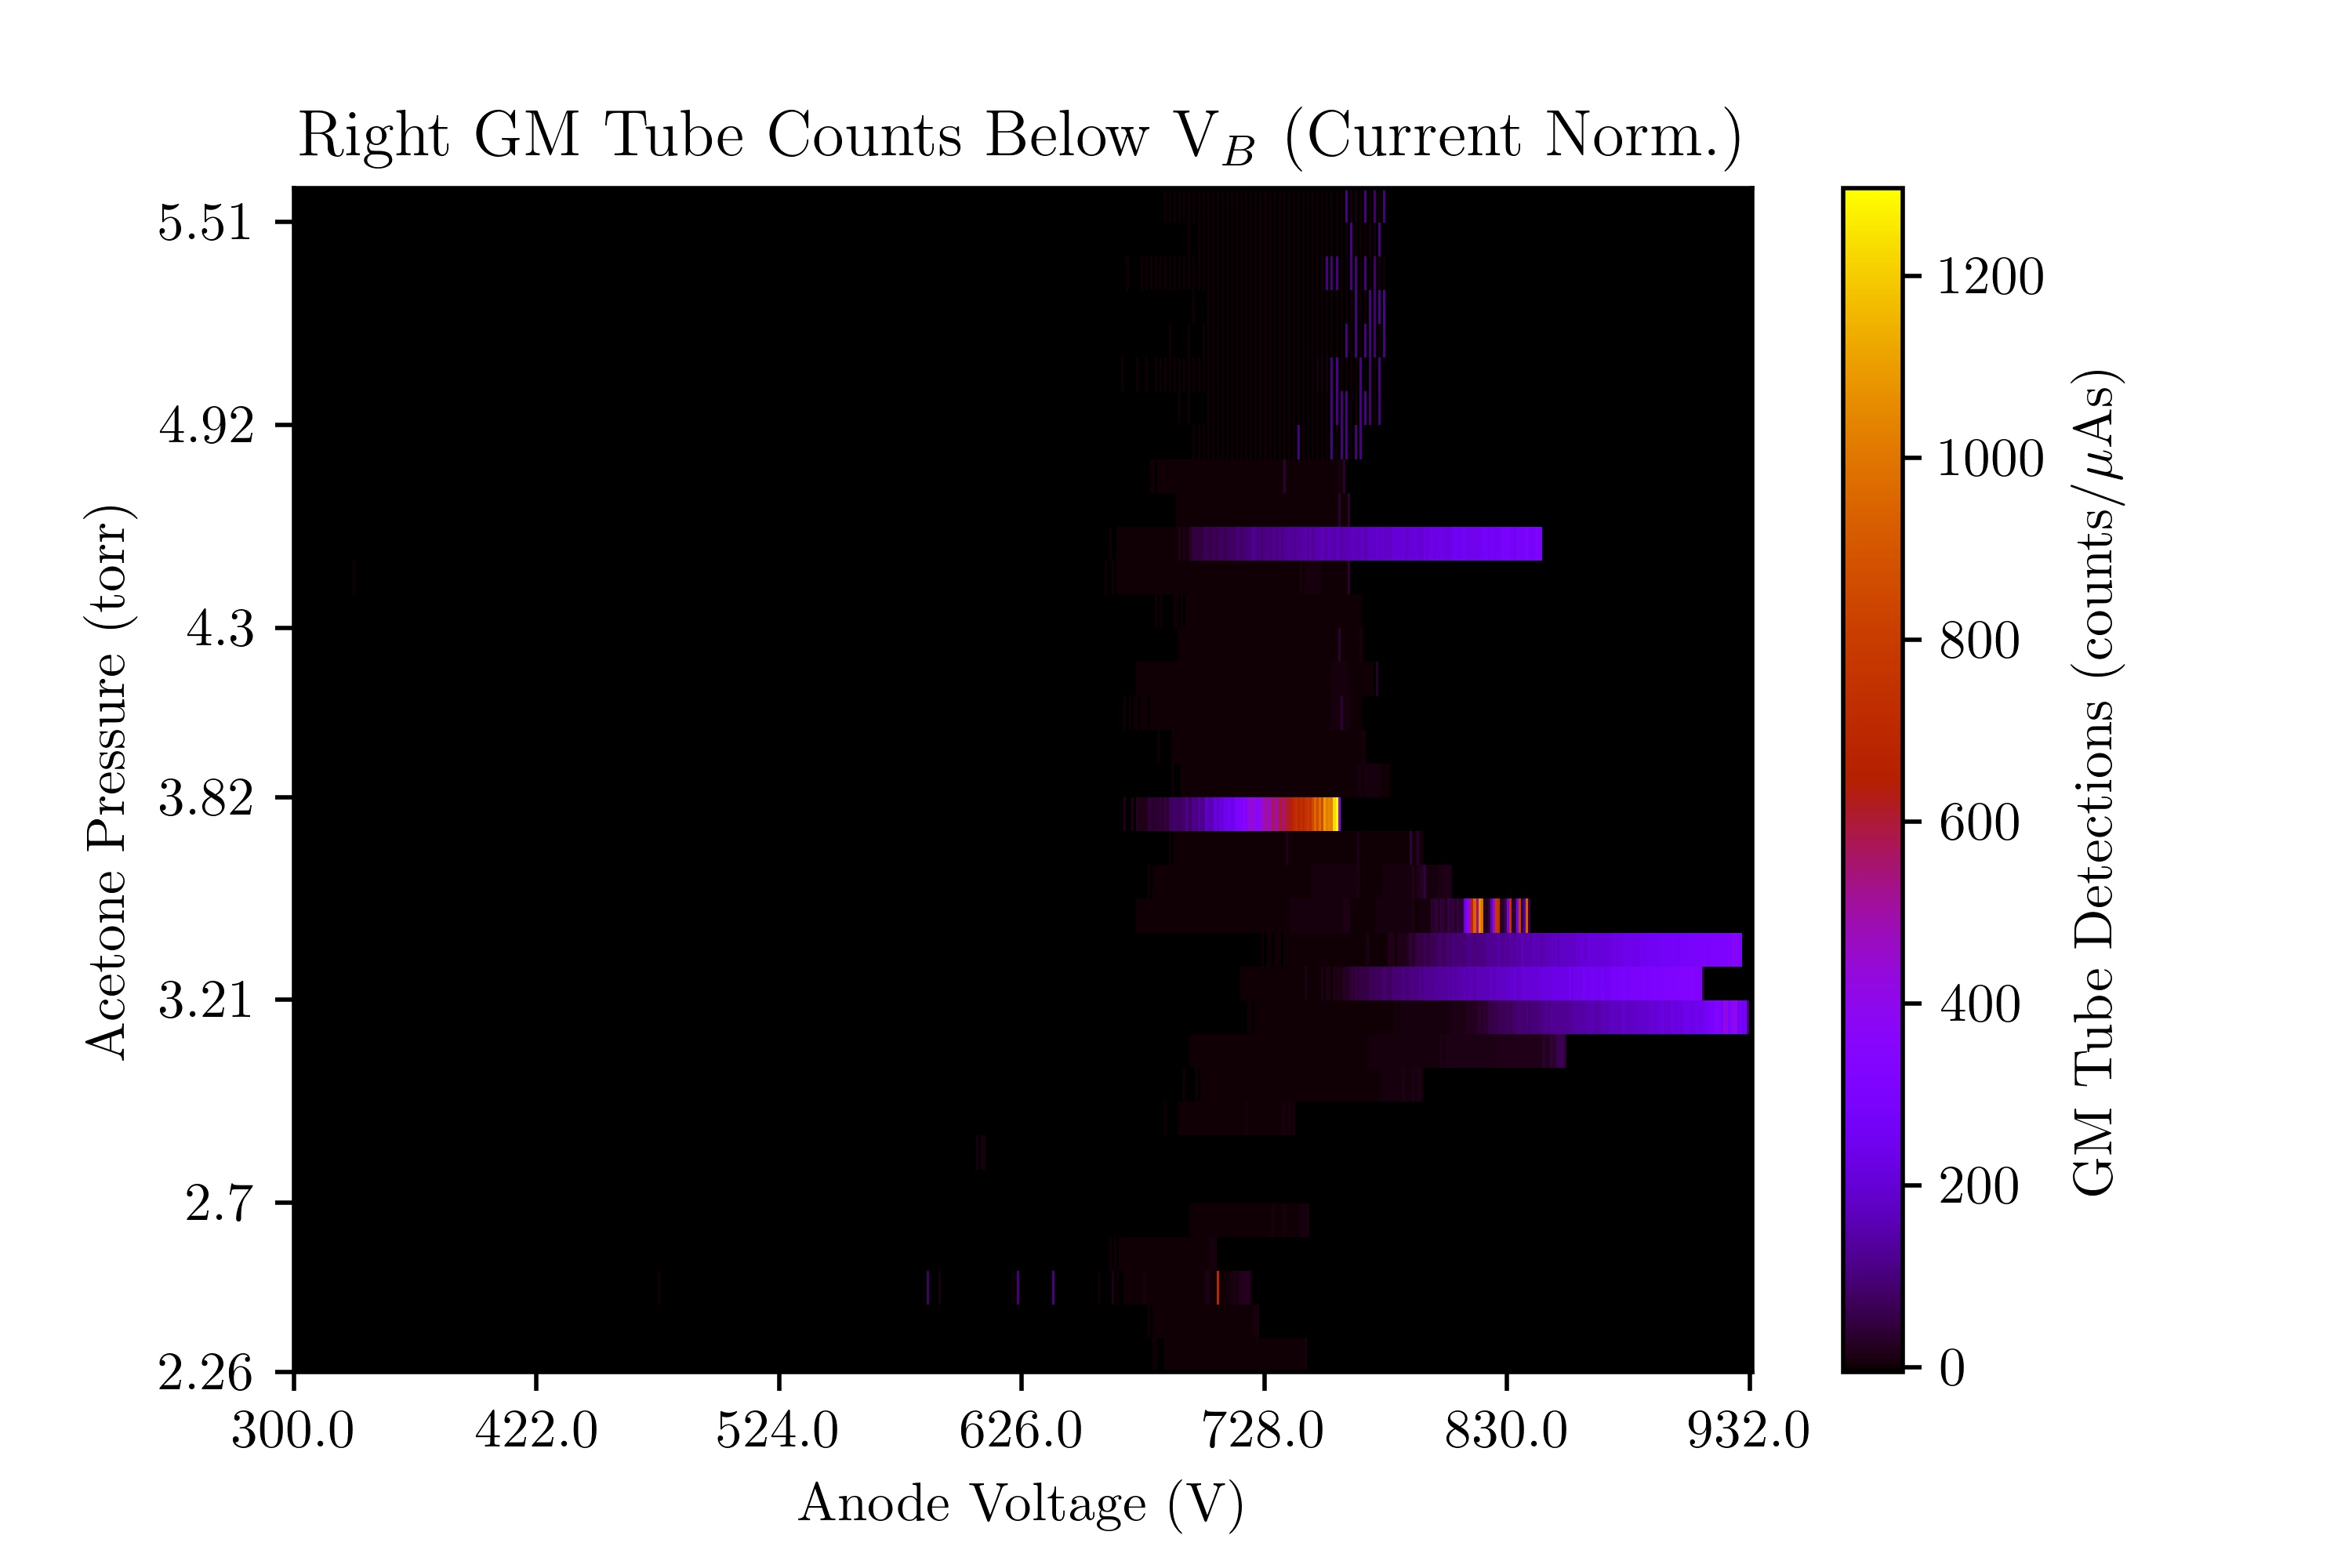
\includegraphics[scale=0.65]{Figs/RGMFinalNorm.jpg}\\
    Optimal pressure is 3.7 torr, optimal anode voltage is 750V
\end{frame}

\begin{frame}{RGM Cont.}
    \centering
    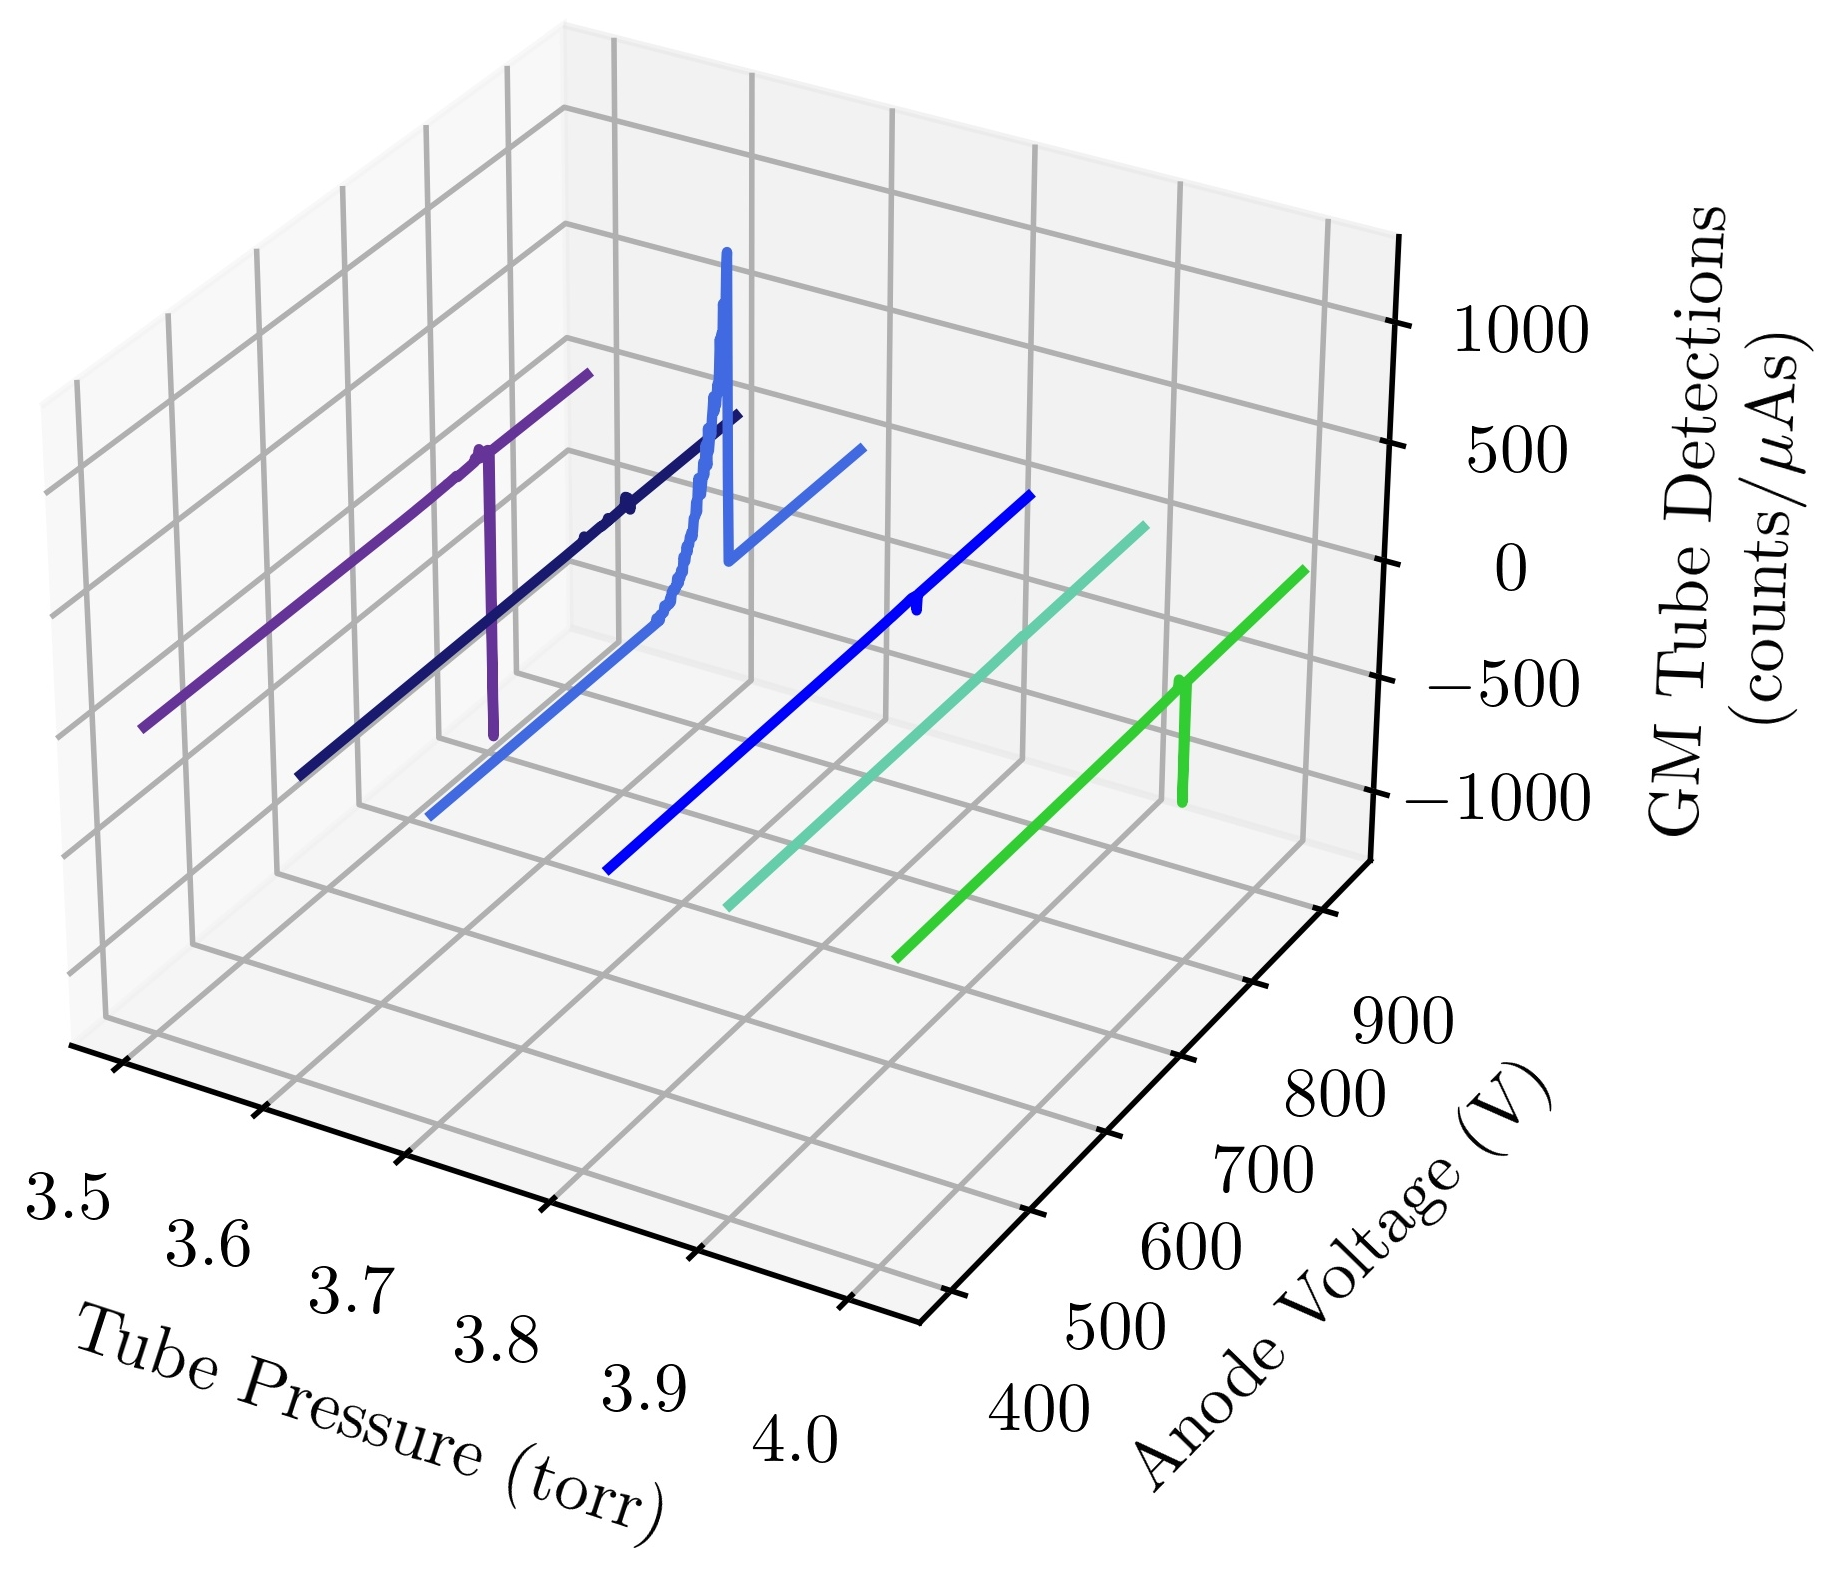
\includegraphics[scale=0.9]{Figs/Plots/RGM Waterfall.jpg}
\end{frame}

\begin{frame}
    \centering
    \vfill
    \Huge\textbf{Thank You}
\end{frame}

\end{document}